\documentclass[class=book, crop=false, oneside, 12pt]{standalone}
\usepackage{standalone}
\usepackage{../../style}
\usepackage[normalem]{ulem}
\graphicspath{{./assets/images/}}

% arara: pdflatex: { synctex: yes, shell: yes }
% arara: latexmk: { clean: partial }
\begin{document}
\chapter{Analisi sintattica: bottom-up parsing}
Iniziamo la trattazione del parsing di tipo \emph{bottom-up}: come suggerisce il nome stesso, consiste nel ricostruire le derivazioni di una parola in ordine inverso, partendo dall'ultima produzione e arrivando infine allo start symbol; a livello visivo, possiamo pensare che la nostra intenzione è di partire dalle foglie di un albero di derivazione e risalirlo fino alla radice.

\section{Classi di grammatiche}
Possiamo subito anticipare che anche per questo approccio possiamo identificare diverse classi di grammatiche, ciascuna delle quali ci permetterà di utilizzare, di volta in volta, diverse tecniche di parsing; in ogni caso, ciascuna di queste classi condivide le seguenti caratterstiche:
\begin{itemize}
    \item per qualsiasi grammatica \(\G\) considerata, andremo sempre a espandere il suo insieme \(\P\) in \(\P'\) aggiungendo la produzione \(S \to S'\), dove \(S'\) è un non-terminale \emph{fresh};
    \item utilizzano i medesimi algoritmi \emph{shift} e \emph{reduce} (ne parleremo più avanti);
    \item hanno sempre un automa a stati finito, detto \emph{automa caratteristico}, il cui ruolo è di supervisionare il funzionamento dell'algoritmo di parsing.
\end{itemize}
Dipendentemente dalla classe di grammatica considerata, avremo automi caratteristici che rappresentano le informazioni in maniera più o meno dettagliata. Maggiore è il livello di dettaglio dell'informazione, più diventa grande e complesso l'automa caratteristico, ma anche più potente diventa il nostro parsing, inteso come numero di diverse grammatiche che può analizzare. Impariamo a conoscere qual è il significato delle abbreviazioni che costituiscono quei nomi un po' criptici delle classi di grammatiche:
\begin{labeling}{LA}
    \item[L] left: leggiamo l'input da sinistra;
    \item[R] ricostruiamo una derivazione rightmost;
    \item[1] andiamo a considerare un simbolo alla volta;
    \item[LA] sta per look ahead;
    \item[S] sta per simple;  
\end{labeling}
Noi diciamo che una grammatica \(\G\) appartiene a una certa classe, ad esempio LR(1), se \(\G\) può essere costruita con la tecnica sottesa al bottom-up parsing di tipo LR(1), vale a dire quando saremo capaci di definire una tabella deterministica che ne rispetti i vincoli.

Tra quelli presentati, il meccanismo più potente è LR(1), complementare di LL(1); per questo motivo noi cercheremo sempre di costruire una tabella di parsing deterministico che rientri nei vincoli di LR(1). Se questo non sarà possibile andremo a scalare in complessità con LALR e SRL.

\section{Un primo esempio di applicazione}
\subsection{Mosse di shift e reduce}
Andiamo a introdurre l'algoritmo che utilizzeremo per verificare se una certa parola appartenga o meno al linguaggio denotato da una certa grammatica, rappresentata dal suo automa caratteristico; questo è detto algoritmo di shift/reduce, dalle due mosse che utilizziamo:
\begin{enumerate}
    \item la mossa di \emph{shift} è quella che compiamo quando passiamo da un nodo (stato) all'altro, inserendo nella pila delle derivazioni parziali il terminale che marca l'arco attraversato e nella pila degli stati il nodo di destinazione;
    \item la mossa di \emph{reduce} è quella che eseguiamo quando raggiungiamo un nodo marchiato da una formula di riduzione (capiremo nell'esempio quale forma hanno) e che ci porta a eliminare dei terminali dalla pila delle derivazioni parziali e degli stati dalla pila degli stati, coerentemente alla struttura dell'automa caratteristico.
\end{enumerate}
Consideriamo come esempio una delle prime grammatiche che abbiamo visto, quella che genera due occorrenze bilanciate:
\begin{equation}
    \label{balanced}
    \G: S \to aSb \mid ab
\end{equation}
\subsection{Esempio di automa}
L'automa caratterisco di tipo LR(1) per questa grammatica è il seguente:
\begin{figure}[H]
    \centering
    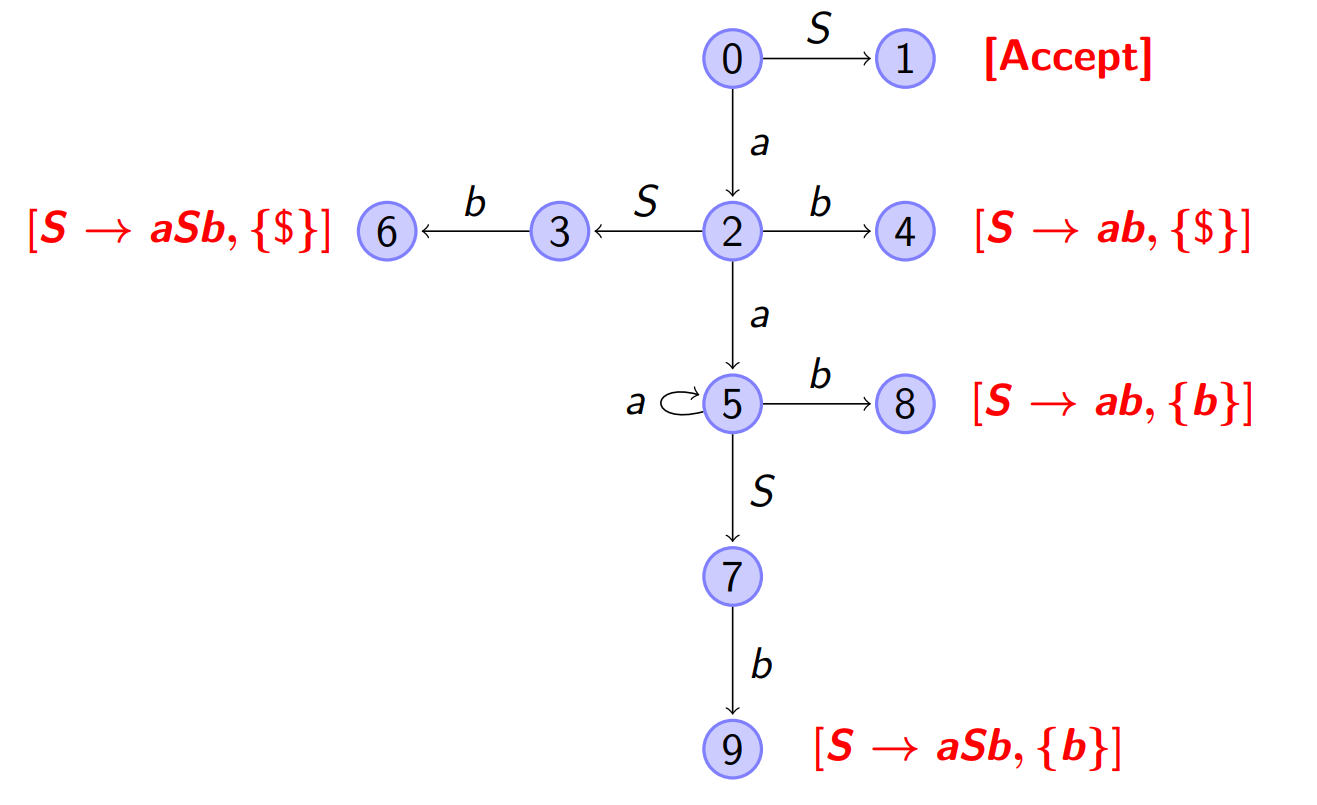
\includegraphics[width=\textwidth,keepaspectratio]{balanced-char_aut-lr1.png}
    \caption{Automa caratteristico LR(1) per Eq. \ref{balanced}}
    \label{balanced-char_aut-lr1}
\end{figure}
Lo utilizzeremo come guida per determinare, di volta in volta, quali mosse di shift e reduce applicare per verificare se una certa parola appartiene o no al linguaggio generato da \(\G\). 

\subsection{Procedura}
Consideriamo ad esempio la parola \(w = aaabbb\). Come prima cosa le applichiamo il carattere terminatore di stringa \(aaabbb\$\). Introduciamo quindi le strutture che utilizzeremo nella procedura, che saranno due pile:
\begin{itemize}
    \item nella prima inseriamo gli stati verso cui ci muoviamo;
    \item nella seconda conserviamo la derivazione parziale a cui siamo arrivati sinora.
\end{itemize}
Si tenga presente che in realtà potremmo farci bastare anche una sola pila, ma andrebbe a complicare sensibilmente la gestione della procedura.
\begin{itemize}
    \item Partiamo dallo stato \(0\) e inseriamolo nella pila degli stati;
    \item il primo simbolo che leggo in \(w\) è \(a\), vedo che l'automa presenta una \(a\)-transizione verso lo stato \(2\), per cui la seguo, inserisco lo stato \(2\) nella pila, passo oltre al simbolo \(a\) appena "consumato" e passo al prossimo simbolo;
    \item il prossimo simbolo è ancora \(a\); di nuovo, seguo la \(a\)-transizione verso lo stato \(5\), lo inserisco nella pila degli stati, passo oltre al simbolo consumato e vado avanti;
    \item abbiamo una terza occorrenza di \(a\) e abbiamo una \(a\)-transizione in forma di self loop in \(5\), che andiamo ad eseguire, reinserendo \(5\) nella pila degli stati passando oltre alla nostra terza \(a\);
    \item troviamo quindi una \(b\), per cui ci spostiamo allo stato \(8\), il quale ha un'etichetta rossa che riporta un passo di riduzione in forma \(S \to ab, \{b\}\); questo sta a indicare che, se abbiamo appena letto il body della produzione, ovvero i due simboli \(ab\), possiamo ritornare indietro di due passi, eliminando i due precedenti stati dalla pila e spostarmi direttamento dal primo \(5\) a \(7\), dal momento che i due stati sono collegati da una \(S\)-transizione:
    \begin{align*}
        \textrm{pila degli stati prima:} &\quad 02558 \\
        \textrm{pila degli stati dopo:} &\quad 0257 
    \end{align*}
    inoltre dobbiamo anche rimuovere gli ultimi due simboli \(ab\) dalla pila della derivazione e sostituirli con \(S\):
    \begin{align*}
        \textrm{pila di derivazione prima:} &\quad \#aaab \\
        \textrm{pila di derivazione dopo:} &\quad \#aaS 
    \end{align*}
    \item leggiamo un'altra \(b\) e avanziamo allo stato \(9\), e anche qui operiamo un passo di riduzione (reduce), nello specifico abbiamo che \(R: S \to aSb, \{b\}\); questo ci dice che dobbiamo tornare indietro di tre passi, eliminando i tre elementi precedenti sia nella pila degli stati e muovendoci verso \(3\), sostituendo nella pila delle derivazioni il body della riduzione con il driver; si osservi attentamente il cambiamento delle pile per capire cosa succede:
    \begin{align*}
        \textrm{pila degli stati prima:} &\quad 02579 & \textrm{pila di derivazione prima:} &\quad \#aaSb \\
        \textrm{pila degli stati dopo:} &\quad 023 & \textrm{pila di derivazione dopo:} &\quad \#aS
    \end{align*}
    \item proseguo quindi con la lettura e incontro una terza \(b\), mi muovo verso \(6\) e incontro una terza riduzione \(R: S \to aSb, \{\$\}\); di nuovo, torno indietro di tre stati e contestualmente sostituisco gli elementi nelle pile: 
    \begin{align*}
        \textrm{pila degli stati prima:} &\quad 0236 & \textrm{pila di derivazione prima:} &\quad \#aSb \\
        \textrm{pila degli stati dopo:} &\quad 0 & \textrm{pila di derivazione dopo:} &\quad \#S
    \end{align*}
    \item abbiamo terminato: ci troviamo nello stato \(0\) e troviamo solamente il nostro start symbol \(S\), che ci permette  muoverci verso lo stato \(1\), e l'endmaker \$; la presenza della keyword \(ACCEPT\) nello stato in cui abbiamo terminato ci indica che la parola è stata riconosciut dall'automa.
\end{itemize}

\subsection{Riassumendo}
Questo è un esempio del procedimento dell'algoritmo di shift/reduce; vediamo quali regole generali possiamo dedurne:
\begin{itemize}
    \item partendo dallo stato iniziale, inizio a leggere la parola data attraversando gli archi marchiati dalle \(symbol\)-transizioni che incontriamo di volta in volta;
    \item quando arrivo in un nodo in cui si dovrà effettuare un passo di riduzione, questo sarà marcato da un'etichetta che avrà la forma \(A \to B, \{l\}\); quello che dovrò fare a questo punto sarà eliminare dalla cima della pila della derivazione il body della riduzione, mettere al suo posto il driver della riduzione, eliminare dalla pila degli stati tanti stati quanti i caratteri nel body della derivazione ed infine inserire nella pila degli stati il nuovo stato che raggiungiamo dal nuovo stato in cima alla pial degli stati con una transizione etichettata con il driver della riduzione.
\end{itemize}
Gli automi caratteristici sono una rappresentazione utile, ma si tenga presente che la stessa funzione può essere ottemperata anche da una tabella.

\section{Costruzione dell'automa}
Dopo aver visto questo esempio, non possiamo fare a meno di domandarci com'è possibile per noi calcolare questo automa caratteristico e la relativa tabella di parsing.

\subsection{Stati}
Andiamo per prima cosa a vedere gli stati. Gli stati sono degli insiemi di items, dove gli items sono oggetti di diverso tipo dipendentemente dalla tecnica di parsing utilizzata:
\begin{labeling}{LR(1)-items}
    \item[LR(0)-items] \(A \to \alpha \cdot \beta\)
    \item[LR(1)-items] [\(A \to \alpha \cdot \beta, L\)], dove \(L \subseteq T \cup \{\$\}\)\footnote{Ricordiamo che \(T\) è l'insieme dei terminali della grammatica considerata.}
\end{labeling}
Da qui capiamo finalmente cosa intendevamo quando prima abbiamo detto che gli LR(1)-items sono più ricchi dei loro equivaleenti LR(0), e ci permettono quindi di riconoscere più grammatiche. Coerentemente alla definzione sopra riportata, avremo che gli automi caratteristici LR(0) sono quelli i cui stati sono LR(0)-items, e analogamente per gli automi carattersitici LR(1).

Andiamo a fare subito un esempio per aiutarci a capire di cosa stiamo parlando. Consideriamo un LR(0)-item \(S' \to \cdot S\): il significato intuitivo è che, se siamo all'inizio della procedura di parsing, siamo in una posizione in cui vogliamo conoscere quali sono le parole derivabili a partire da \(S\), per cui è logico pensare che il nostro item \(S' \to \cdot S\) debba stare nello stato iniziale dell'automa, che chiamiamo \(P_0\).

Ma non sarà l'unico item a risiedere in \(P_0\). Per aiutarci, riprendiamo la nostra fidata grammatica in Eq. \ref{balanced}: in questo caso, analizzare la parola vuol dire aspettarsi qualcosa che derivi da \(aSb\) oppure \(ab\), per cui gli LR(0)-items di \(S\) saranno:
\begin{itemize}
    \item \(S \to \cdot aSb\);
    \item \(S \to \cdot ab\).
\end{itemize}
E verranno inseriti in \(P_0\).

\subsection{Chiusura di un insieme di LR(0)-items}
Andiamo ora a vedere il concetto di chiusura di un insieme di LR(0)-items:

\begin{definition}
    Sia \(P\) un insieme di LR(0)-items; allora, \(closure_0(P)\) è il più piccolo insieme che soddisfa la seguente equazione:
    \begin{equation}
        closure_0(P) = P \cup \{B \to \cdot \gamma \; \mid \; A \to \alpha \cdot B \beta \in closure_0(P) \; \textrm{e} \; B \to \gamma \in P'\}
    \end{equation}
\end{definition}

La chiusura consiste sostanzialmente nell'aggiungere, per tutti quegli items che hanno un punto davanti ad un non-terminale, tutte le derivazioni possibili di quel non-terminale; questo va applicato ricorsivamente fino a che non sono presenti tutte le chiusure delle produizioni con un punto davanti ad un non-terminale. Più facile a farsi che a dirsi, credetemi.

\subsection{Esempio di calcolo della chiusura}
Prendiamo ora ad esempio la seguente grammatica:
\begin{align*}
    E &\to E+T \mid T\\
    T &\to T*F \mid F\\
    F &\to (E) \mid id
\end{align*}
e calcoliamo \(closure_0(\{E' \to \cdot E\})\). Ecco il procedimento passo per passo:
\begin{enumerate}
    \item inizializziamo \(closure_0(\{E' \to \cdot E\})\) = \(\{E' \to \cdot E\}\); 
    \item andiamo a vedere se questo insieme contiene qualche marker davanti ad un non-terminale: effettivamente, c'è un marker prima di \(E\);
    \item aggiungiamo quindi le due produzioni di \(E\) alla chiusura \(\{E \to \cdot E+T\}\) e \(\{E \to \cdot T\}\);
    \item una volta aggiunte queste produzioni, vediamo ricorsivamente se si presentano altre situazioni con \(\cdot\) prima di un non-terminale;
    \item nel primo caso troviamo ancora \(\cdot E\), che però abbiamo già analizzato;
    \item nel secondo caso invece abbiamo \(\cdot T\) e non abbiamo ancora analizzato tutte le produzioni di \(T\), quindi andiamo ad aggiungere all'insieme le produzioni di \(T\);
    \item aggiungamo \(\{T \to \cdot T * F\}\) e \(\{T \to \cdot F\}\);
    \item ci troviamo di nuovo in un caso in cui abbiamo due nuove derivazioni con \(\cdot\) davanti
    a un non-terminale, ma \(\cdot T\) è già analizzato, per cui analizziamo solo \(\cdot F\);
    \item aggiungiamo le produzioni di \(F\): \(\{F \to \cdot (E)\}\) e \(\{F \to \cdot id \}\);
    \item siamo arrivati alla conclusione, e qui sotto è riportato l'insieme chiusura che abbiamo trovato:
\end{enumerate}
\begin{align*}
    E' &\to \cdot E \\
    E  &\to \cdot E+T \\
    E  &\to \cdot T \\
    T  &\to \cdot T * F \\
    T  &\to \cdot F \\
    F  &\to \cdot (E) \\
    F  &\to \cdot id
\end{align*}

Ora che abbiamo visto un applicazione otteniamo lo pseudocodice dell'algoritmo per la computazione della chiusura:
\begin{figure}[H]
    \centering
    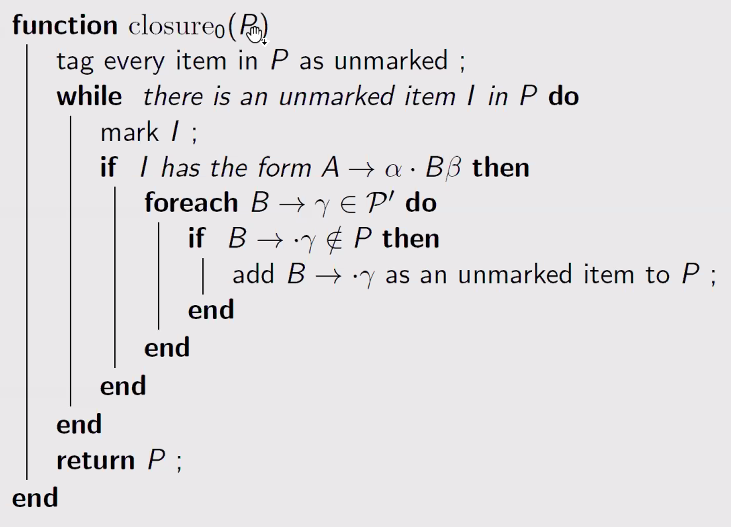
\includegraphics[width=.8\textwidth]{bottom-up-parsing_closure_algorithm.png}
    \caption{Algoritmo per il calcolo di \(closure_0(P)\)}
\end{figure}
\subimport{assets/pseudocode/}{lr0-closure.tex}

\subsection{Costruire un automa caratteristico per il parsing LR(0)}
Vedremo ora come costruire un automa caratteristico per il parsing di tipo LR(0) data una certa grammatica. La tecnica di costruzione è incrementale: andiamo a popolare un set di stati definendo mano a mano la funzione di transizione, fino a saturazione; il lettore si accorgerà che tale tecnica è poi utilizzata per costruire anche altri automi LR.

\paragraph{Inizio}
In primis, definiamo il kernel dello stato iniziale come \(P_0 = \{S' \to \cdot S\}\), dove \(S'\) è un carattere inserito da noi, mentre \(S\) è lo start symbol della nostra grammatica.

\paragraph{Svolgimento}
Fino a che non esauriamo gli stati ancora da visitare andiamo a prenderli uno alla volta e li analizziamo nel segiente modo:
\begin{enumerate}
    \item calcoliamo il la chiusura del kernel dello stato, questo insieme rappresenta tutte le produzioni che si possono usare da un certo stato per transitare verso altri stati;
    \item una volta calcolata la chiusura del kernel le produzioni (gli item) che abbiamo già collezionato avranno forma \(A \to \alpha \cdot x \beta\), il che significa che nello stato in cui mi trovo, diciamo \(P\), ho già visto \(\alpha\) e posso fare una transizione a \(x\beta\);
    \item esiste quindi una transizione da \(P\) a uno stato \(P'\) attraverso l'item \(A \to \alpha x \cdot \beta\); se \(x\) è un terminale, tale transizione rappresenta un'operazione di shift (come abbiamo visto nell'esercizio della sezione scorsa). Questo significa che avrò una transizione etichettata con \(x\) che mi porta da \(P\) a \(P'\);
    \item a questo punto genero il nuovo stato \(P'\) che contiene come kernel l'item \(A \to \alpha x \cdot \beta\), ricordando che poi andrò a includere tra gli item di \(P'\) anche gli item che appartengono a \(closure_0 (\{ A \to \alpha x \cdot \beta \})\), poiché se \(\beta\) è un non-terminale allora mi aspetto di poter trovare in \(P'\) anche tutto ciò che deriva da \(\beta\).
\end{enumerate}
C'è però una nota da aggiungere a questo procedimento: può accadere che quando generiamo un nuovo stato \(P'\) per transizione da uno stato \(P\) ci rendiamo conto che il kernel di questo stato corrisponde al kernel di un altro stato che abbiamo già vistisato, diciamo \(Q\); in questo caso invece che creare un nuovo stato \(P'\), quello che facciamo è collegare (tramite una \(x\)-transizione) \(P\) a \(Q\).

\subsubsection{Esempio costruzione automa caratteristico LR(0)}
\label{esercizio_costruzione_automa_lr0}
Per consolidare la procedura sopra illustrata, andiamo subitoa a metterele mani su un esempio di costruzione di un automa caratteristico per il parsing LR(0), in particolare per la seguente grammatica:
\begin{align*}
    S &\to aABe \\
    A &\to Abc \mid b \\
    B &\to d
\end{align*}

\paragraph{Inizio}
Partiamo creando lo stato iniziale, lo stato \(0\):
\begin{equation*}
    S' \to \cdot S
\end{equation*}
Ma c'è di più: nello stato iniziale va inserita anche la \(closure_0(\{ S' \to \cdot S \})\), quindi aggiungo le produzioni di \(S\): \(S \to \cdot aABe\). Dato che non sono presenti altre produzioni con marker prima di caratteri non-terminali, lo stato \(0\) è completo.

\paragraph{Svolgimento}
A questo punto ci troviamo nello stato \(0\) ed abbiamo due produzioni, una con il marker prima di \(S\) ed una con il marker prima di \(a\), per cui dobbiamo aggiungere i seguenti due stati:
\begin{enumerate}
    \item \(\tau (0, S) = 1\)
    \item \(\tau (0, a) = 2\)
\end{enumerate}
Nota: gli stati possono venire indicati con la notazione :
\begin{equation*}
    \tau( \textrm{stato di provenienza}, \textrm{transizione di provenienza}).
\end{equation*}
Questi stati però potrebbero essere già presenti! Non è questo il caso dato che sono i primi stati che troviamo, ma in seguito dovremmo ricordarci di tale controllo. \\

Partiamo con l'analizzare il nuovo stato \(\tau (0, S) =\) 1. \\
Dobbiamo calcolare il \emph{kernel} dello stato, che si ottiene spostando il marker oltre al carattere che ci ha portati qui:
\begin{equation*}
    S' \to S \cdot
\end{equation*}
Questo è quello che viene definito kernel dello stato; non presenta ulteriori transizioni possibili dato che il marker è arrivato in fondo, quindi passiamo ad analizzare un altro stato. \\

Andiamo ad analizzare lo \(\tau (0, a) =\) 2. \\
Il kernel questa volta è:
\begin{equation*}
    S \to a \cdot ABe
\end{equation*}
Dato che il kernel presenta almeno una produzione con un non-terminale alla destra del marker, dobbiamo aggiungere la chiusura del kernel a questo stato, ovvero:
\begin{align*}
    A &\to \cdot Abc\\
	A &\to \cdot b
\end{align*}
Quindi gli item dello stato 2 sono:
\begin{align*}
    S &\to a \cdot ABe\\
    A &\to \cdot Abc\\
	A &\to \cdot b
\end{align*}
Dallo stato 2 avremo quindi due possibili transizioni, una tramite \(A\) ed una tramite \(b\). \\

Partiamo ad analizzare \(\tau (2, A) = 3\). \\
Il kernel di questo stato è composto da due produzioni, dato che da \(2\) si può arrivare in \(3\) tramite due distinte produzioni:
\begin{align*}
    S &\to aA \cdot Be \\
    A &\to A \cdot bc
\end{align*}
Per verificare se questo stato è già stato raggiunto, vado a verificare che non siano presenti stati con gli stessi item; in questo casp non ce ne sono, per cui lo stato \(3\) non è ancora stato effettivamente aggiunto e quindi lo tengo.

Calcoliamo la chiusura dello stato, che ci porta ad aggiungere la seguente produzione:
\begin{equation*}
    B \to \cdot d
\end{equation*}
Una volta calcolata la chiusura, mi segno i nuovi stati da visitare.
\begin{itemize}
    \item \(\tau (3, B) = 5\)
    \item \(\tau (3, b) = 6\)
    \item \(\tau (3, d) = 7\)
\end{itemize}

Analizziamo ora lo stato \(\tau (2, b) = 4\). \\
Questo stato ha come kernel:
\begin{equation*}
    A \to b \cdot
\end{equation*}
e non presenta ulteriori possibili sviluppi, quindi passiamo oltre. \\

Analizziamo lo stato \(\tau (3, B) = 5\). \\
Il kernel in questo caso è:
\begin{equation*}
    S \to aAB \cdot e
\end{equation*}
questo kernel è già chiuso (la sua chiusura, infatti, è un insieme vuoto) e ci offre come unica transizione possibile \(\tau (5, e) = 8\). \\

Analizziamo lo stato \(\tau (3, B) = 6\). \\
Il kernel in questo caso è:
\begin{equation*}
    A \to Ab \cdot c
\end{equation*}
Anche questo kernel è già chiuso; ci offre la transizion allo stato \(\tau (6, c) = 9\). \\

Analizziamo lo stato \(\tau (3, d) = 7\). \\
Questo stato ha come kernel:
\begin{equation*}
    B \to d \cdot 
\end{equation*}
Tale kernel è chiuso e non presnta transizioni uscenti. \\

Non ci rimane che analizzare gli stati \(8\) e \(9\) che presentano rispettivamente i seguenti kernel:
\begin{align*}
    S &\to aABe \cdot \\
    A &\to Abc \cdot
\end{align*}
questi due kernel non presentano ulteriori transizioni.

\paragraph{Conclusione}
In conclusione, l'automa caratteristico che otteniamo da questo procedimento può essere visualizzato in Fig.\ref{charateristic-automata_cosntruction}
\begin{figure}
    \centering
    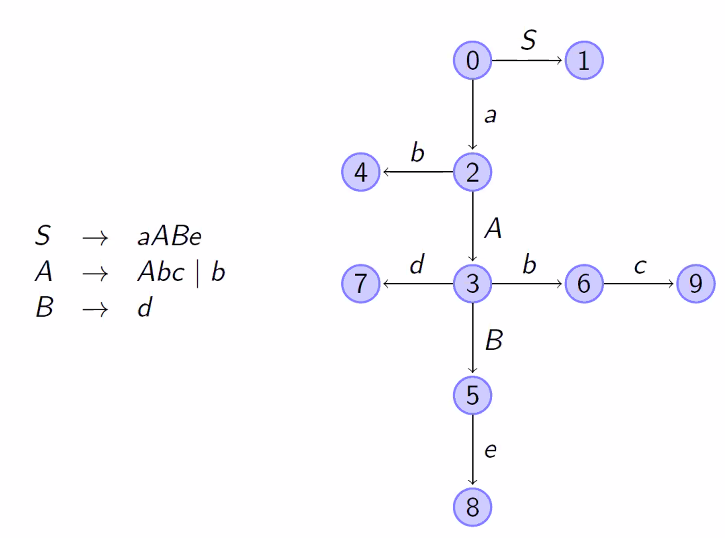
\includegraphics[width=.8\textwidth]{charateristic-automata_cosntruction.png}
    \caption{Automa caratteristico LR(0) per la grammatica \ref{esercizio_costruzione_automa_lr0}}
    \label{charateristic-automata_cosntruction}    
\end{figure}

Una volta terminata questa arzigogolata esercitazione possiamo dare un'occhiata all'algoritmo per la costruzione di un automa LR(0) in Alg.\ref{alg:char-automata}. \\
\begin{figure}
    \centering
    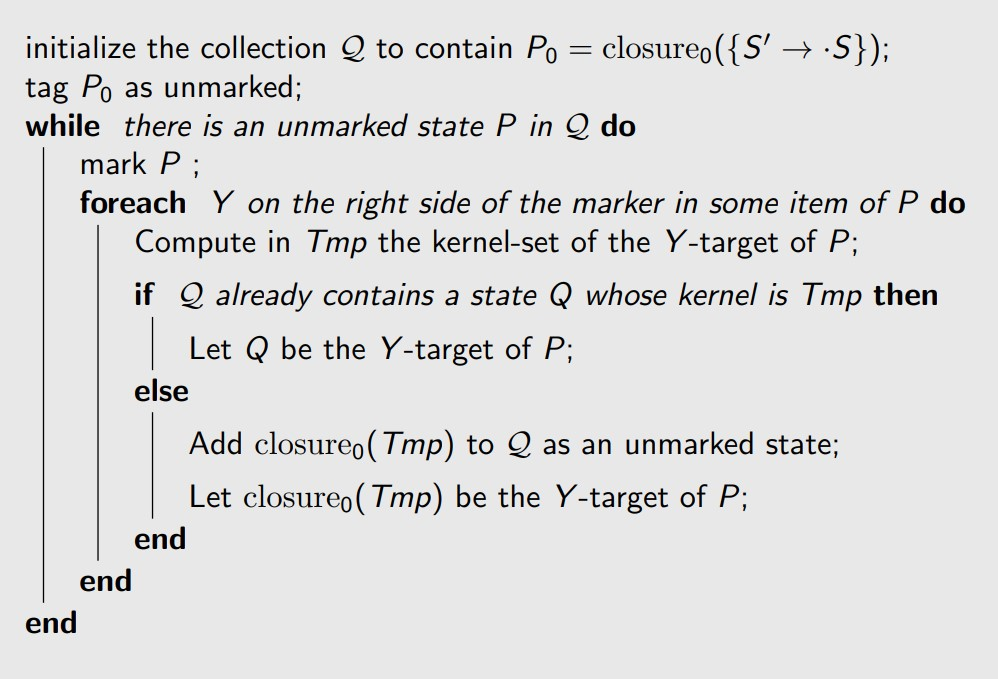
\includegraphics[width=.8\textwidth]{lr0-automata_construction_algorithm.jpg}
    \caption{Algoritmo per la costruzione di un automa LR(0)}
    \label{lr0-automata_construction_algorithm}    
\end{figure}
\subimport{assets/pseudocode/}{char-automata.tex}

Ma dove sono finite le etichette rosse che sull'automa dell'esercizio di shift/reduce ci segnalavano le mosse di reduce? Lo scopriremo nella prossima sezione.

\section{Parsing table per bottom-up}
L'algoritmo di shift/reduce compie delle mosse in base a cosa leggiamo sulle due pile (pila del parsing e pila della lettura). L'algoritmo usa una tabella di parsing per muoversi. La tabella ha tante righe quanti gli stati dell'automa caratteristico, ed una colonna per ogni simbolo in \(V \cup \{ \$ \}\). Nota che la tabella dipende dall'automa caratteristico, automi diversi portano a tabelle diverse che portano a tipi di parsing diversi.

Le mosse di shift dipendono direttamente dalla funzione di transizione dell'automa, mentre le mosse di reduce sono più articolate: vanno effettuate solo quando raggiungiamo quei particolari stati etichettati ed implicano poi che dobbiamo cancellare degli elementi dalla pila degli stati e dalla pila di lettura per poi inserire altri caratteri in quest'ultima pila.

Le mosse di reduce dipendono dal contenuto degli stati dell'automa: in un certo stato della tabella di parsing andiamo ad inserire una mossa di riduzione se la produzione \(A \to \beta\) è effettuata in uno stato contenente un reducing item per \(A \to \beta\). A questo punto però ci chiediamo: cosa sono i reducing item?
\begin{itemize}
    \item Item \(A \to \beta \cdot \) nel caso di LR(0)-items, ovvero quando sono arrivato alla fine della produzione di \(\beta\);
    \item item \(A \to \beta \cdot, \; \Delta\) nel caso LR(1)-items, ovvero quando ho terminato l'analisi del body di \(\beta\).
\end{itemize}
Le riduzioni dipendono dalla \emph{lookahead function} \(\mathcal{LA}\), la quale è definita per tutte le coppie \((P,\; A \to \beta)\) tali che \(P\) contiene un reducing item per \(A \to \beta\).

Da menzionare il fatto che la scelta dell'automa e della lookahead function per la costruzione della parsing table sono le caratteristiche che distinguono le varie tecniche di bottomup parsing. Nello specifico abbiamo le seguenti conseguenze:
\begin{itemize}
    \item la classe delle grammatiche analizzabili dipende dalla scelta appena menzionata;
    \item anche la dimensione della parsing table dipende da tale scelta;
    \item la procedura di riempimento della parsiing table è invece indipendente;
    \item anche l'algoritmo di parsing è sempre uguale.
\end{itemize}

\subsection{Costruire una parsing table per il bottom-up parsing}

Vediamo ora nello specifico come costruire una parsing table. Dobbiamo riempire ogni entry \((P, Y)\) seconndo le seguenti regole:
\begin{itemize}
    \item se \(Y\) è un terminale e \(\tau (P,Y) = Q\) inserisci la mossa \texttt{shift} Q;
    \item se \(P\) contiene un reducing item per \(A \to \beta\) e \(Y \in \mathcal{LA}(P, A \to \beta)\), inserisci la mossa \texttt{reduce} \(A \to \beta\);
    \item se \(P\) contiene l'accepting item e \(Y=\$\) inserisci \texttt{accept};
        \begin{itemize}
            \item nel caso degli automi LR(0) l'item è \(\{S' \to S \cdot\}\);
            \item nel caso degli automi LR(1) l'item è \(\{S' \to S \cdot, \; \Delta\}\);
        \end{itemize}
\item se \(Y\) è un terminale o \$ e nessuna delle condizioni precedenti è valida, inserisce \texttt{errore};
    \item se \(Y\) è un non-terminale e \(\tau (P, Y) = Q\) inserisci la mossa \texttt{goto} \(Q\).
\end{itemize}

\subsection{Conflitti}
L'informazione che è contenuta nella tabella di parsing in posizione \(M[P, Y]\) viene dunque utilizzata per stabilire che tipo di operazione effettuare, dipendentemente dallo stato \(P\) in cui ci troviamo e dal simbolo \(Y\), terminale o non-terminale che esso sia.
Nonostante la grandezza della parsing table dipenda dal tipo di algoritmo di parsing bottom-up che andiamo ad applicare (quindi SLR(1), LALR(1), LR(1)) e dalla funzione di lookahead (\(\mathcal{LA}\)), l'algoritmo che viene utilizzato per riempire la tabella rimane quello visto in precedenza.

Visto che abbiamo già potuto modo di discutere di tabelle di parsing anche per il parsing di tipo top-down, risulta naturale metterle a confronto e chiedersi se, anche in questo caso, sia possibile ottenere dei \textbf{conflitti} (ovvero delle entries multiple defined). Questa situazione può verificarsi anche in questo caso in due differenti modalità: parleremo di
\begin{itemize}
    \item \textbf{s/r conflict} (o shift/reduce conflict) nel caso in cui almeno un entry della tabella di parsing contenga sia un'operazione di \texttt{shift} Q (data dal fatto che esiste una \(Y\)-transizione che va dallo stato \(P\), dove ci troviamo attualmente, allo stato \(Q\)), sia un'operazione di \texttt{reduce} \(A \rightarrow \beta\) (poiché \(P\) contiene un reducing item per \(A \rightarrow \beta\) e \(Y \in \mathcal{LA}(P, A \rightarrow \beta)\));
    \item \textbf{r/r conflict} (o reduce/reduce conflict) nel caso in cui almeno un entry della tabella di parsing contenga due operazioni di \texttt{reduce} per produzioni distinte.
\end{itemize}

La prossima domanda sorge spontanea: cosa accade quando abbiamo un conflitto? La conclusione che possiamo trarre è che, se stiamo eseguendo un parsing di un certo tipo (ad esempio SLR(1), LALR(1) o LR(1)) per una grammatica \(\G\) e troviamo un conflitto mentre costruiamo la tabella, allora \(\G\) \emph{non} è una grammatica di quel particolare tipo.
% La prossima domanda sorge spontanea: cosa accade al parsing quando abbiamo un conflitto? Visto che nell'ambito del parsing bottom-up abbiamo già parlato di tre differenti classi di grammatiche, prendiamoci del tempo per analizzare ogni caso singolarmente: se troviamo almeno un conflitto in una tabella di parsing costruita per la grammatica \(\G\) per eseguire un parsing di tipo 
% \begin{itemize}
%     \item \(SLR(1)\), allora \(\G\) \textbf{non} è una grammatica \(SLR(1)\)
%     \item \(LALR(1)\), allora \(\G\) \textbf{non} è una grammatica \(LALR(1)\)
%     \item \(LR(1)\), allora \(\G\) \textbf{non} è una grammatica \(LR(1)\)
% \end{itemize}
\section{Tabelle di Parsing SLR(1)}
Il parsing di tipo \(SLR(1)\) è un parsing meno raffinato, in quanto le tabelle contengono meno informazioni; questo è per due motivi:
\begin{enumerate}
    \item la loro costruzione ha come base di partenza un automa caratteristico con LR(0)-item;
    \item la funzione di lookahead è pari a \(\mathcal{LA}(P, A \rightarrow \beta) = follow(A)\) per ogni \(A \rightarrow \beta \cdot \in P\).
\end{enumerate}
Come già detto precedentemente, una grammatica \(\G\) è SLR(1) se e solo se la parsing table ottenuta non ha conflitti.

\subsection{Esempio costruzione tabella di parsing SLR(1)}
Dobbiamo costruire la tabella di parsing \(SLR(1)\) per la seguente grammatica \(\G\):
\begin{align*}
    S &\rightarrow aABe \\
    A &\rightarrow Abc \mid b \\
    B &\rightarrow d
\end{align*}
Riconoscerete di certo questa grammatica, l'abbiamo già vista nella costruzione dell'automa caratteristico. Tuttavia, il nostro obiettivo qui è costruire la tabella di parsing, e per farlo utilizzeremo i risultati ottenuti in precedenza: sappiamo infatti che lo stato \(1\) (anche indicato dal colore verde) è quello che contiene l'\textbf{Accepting Item}, mentre invece gli stati contenenti i \textbf{Reducing Item} (segnalati come stati finali) sono invece 4, 7, 8, 9 (si osservi Fig.\ref{fig:charateristic-automata-complete}). 
\begin{figure}
    \centering
    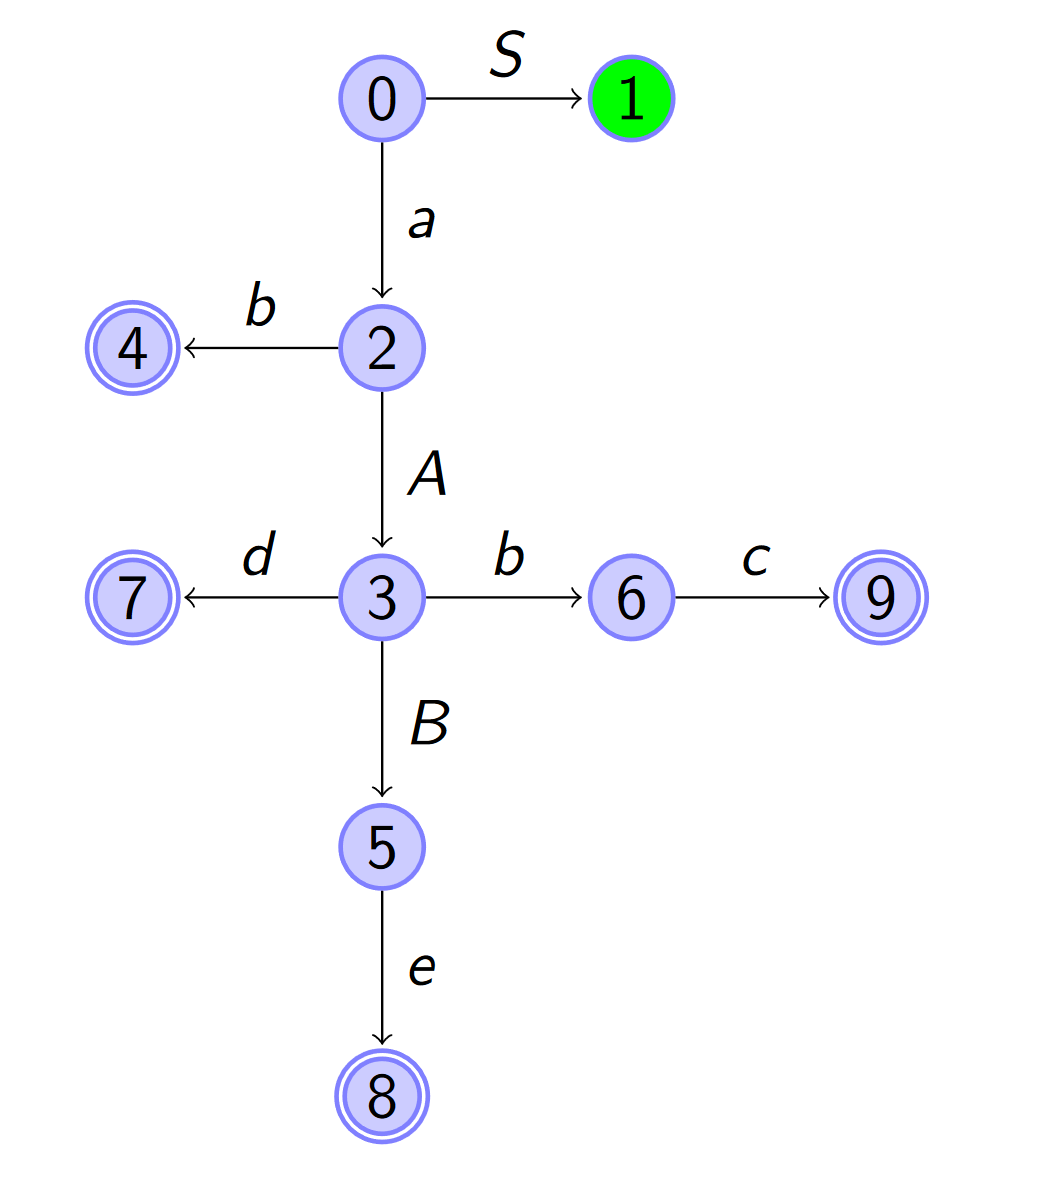
\includegraphics[width=.8\textwidth]{charateristic-automata-complete.png}
    \caption{Automa Caratteristico per la Bottom-Up Parsing Table}
    \label{fig:charateristic-automata-complete}    
\end{figure}
In particolare, possiamo dire che i reducing item sono:
\begin{enumerate}
    \item \(\{A \rightarrow b \cdot\}\) per lo stato 4;
    \item \(\{B \rightarrow d \cdot\}\) per lo stato 7;
    \item \(\{S \rightarrow aABe \cdot\}\) per lo stato 8;
    \item \(\{A \rightarrow Abc \cdot\}\) per lo stato 9;
\end{enumerate}
Avendo a disposizione l'automa caratteristico e i dati sopra citati è dunque possibile costruire la tabella di parsing seguendo l'algoritmo per la costruzione di una tabella di parsing per il bottom-up parsing (ricordiamo all'utente distratto che siamo nell'ambito del parsing; parsing e chiudoing). Procediamo quindi in questo modo:
\begin{enumerate}
    \item creiamo una tabella con tante righe quanti sono gli stati nel nostro automa caratteristico (in questo caso da 0 a 9) e con tante colonne quanti sono i terminali (a cui va aggiunto il \$) e i non-terminali presenti all'interno della nostra grammatica (in questo caso abbiamo di conseguenza \emph{a b c d e \$ A B S});
    \item facendo riferimento all'automa caratteristico, se \(Y\) è un terminale e c'è una transizione \(\tau (P, Y) = Q\) (ovvero una transizione che va dallo stato \(P\) allo stato \(Q\) attraversando un arco con etichetta \(Y\)), allora inseriamo un'operazione di \texttt{shift} \(Q\) nella cella \(M[P, Y]\); ad esempio, nel nostro caso inseriremo \(M[0, a] = 2\);
    \item A questo punto è necessario calcolare i follow (e di conseguenza i first, Tab.\ref{tab:first-follow-SLR(1)parsing}), in quanto per poter inserire correttamente le operazioni di \texttt{reduce} abbiamo bisogno di avere queste informazioni per la funzione di lookahead (\(\mathcal{LA}\));
\begin{table}[H]
    \centering
    \subimport{assets/tables/}{ptbu-follow.tex}
    \caption{LRS(1) Parsing Table - Calcolo Follow per Lookahead}
    \label{tab:first-follow-SLR(1)parsing}
\end{table}
    \item Una volta calcolati i follow è possibile inserire un'operazione di \texttt{reduce} \(A \rightarrow \beta\) in \(M[P, Y]\) nel caso in cui \(P\) sia un stato contenente un reducing item (quindi nel nostro caso sia uno tra 4, 7, 8 o 9) e per tutti quei terminali \(Y \in \mathcal{LA}(P, A \rightarrow \beta) = follow(A)\) (e.g. \(M[4, b] = A \rightarrow b\) in quanto \(A \rightarrow b \cdot\) è un reducing item per lo stato 4 e \(b \in follow(A)\))
    \item Inseriamo in posizione \(M[1, \$]\) l'operazione di \texttt{Accept}, in quanto 1 contiene un accepting item;
    \item A questo punto dovremmo valorizzare a \texttt{error} tutte quelle celle \(M[P, Y]\) dove \(Y\) è o \$ o un terminale che non ricade nei casi precedenti; tuttavia per una maggiore comprensione a livello visivo, nel nostro esempio queste celle verranno lasciate vuote;
    \item Infine, inseriamo un'operazione del tipo \texttt{goto} \(Q\) per tutti quelle celle \(M[P, Y]\) dove \(Y\) è un non-terminale e per cui esiste una transizione \(\tau(P, Y) = Q\) (ad esempio \(M[0, S]\) = \texttt{goto} 1, come è anche osservabile dall'automa caratteristico).
\end{enumerate}
In Tab.\ref{tab:parsing-table-SLR(1)parsing} possiamo trovare il risultato finale dell'algoritmo. Ai fini di una corretta lettura della tabella, specifichiamo qui sotto alcune convenzioni che verranno impiegate per motivi di [convenienza?], come ad esempio:
\begin{itemize}
    \item l'operazione di \texttt{shift} \(Q\) verrà indicata con \(sQ\);
    \item l'operazione di \texttt{reduce} \(A \rightarrow \beta\) con \(rK\), dove \(K\) indica la \(K\)-esima produzione della grammatica;
    \item \emph{Acc} indica l'accepting item;
    \item l'operazione di \texttt{Goto} \(Q\) verrà indicata semplicemente da Q.
\end{itemize}
\begin{table}[H]
    \centering
    \subimport{assets/tables/}{ptbu-complete.tex}
    \caption{LRS(1) Parsing Table}
    \label{tab:parsing-table-SLR(1)parsing}
\end{table}
Specifichiamo quindi per chiarezza il significato dei vari \(rK\):
\begin{itemize}
    \item \(r1 = S \to aABe\)
    \item \(r2 = A \to Abc\)
    \item \(r3 = A \to b\)
    \item \(r4 = B \to d\)
\end{itemize}

Dal momento che \(\G\) dà origine a una nuova grammatica senza creare alcun conflitto, possiamo concludere che \(\G\) è SLR(1).

Prima di passare alla prossima sezione è necessario precisare che \emph{solamente} le celle vuote che hanno per colonna un terminale o \$ sarebbero valorizzate a \texttt{error}: infatti, le celle vuote che hanno per colonna un non-terminale rimangono semplicemente vuote, in quanto sono dei casi che non è possibile che si verifichino. 

\subsection{Algoritmo Shift/Reduce}
\begin{itemize}
    \item \textbf{Input}: una stringa \(w\) e la tabella di parsing \(M\) per \(\G = (V, T, S, \P)\);
    \item \textbf{Output}: una derivazione di \(w\) in ordine inverso se \(w \in \mathcal{L}(\G)\) (per trovare i passi di derivazione che ci portano a \(w\) dovremo leggere tutte le reduce che abbiamo applivato in ordine inverso); otterremo invece \texttt{error} se \(w \notin \mathcal{L}(\G)\);
    \item \textbf{Inizializzazione}: Per l'algoritmo è necessario inserire all'interno dell'input buffer la stringa \(w\$\), e inoltre abbiamo bisogno di due strutture dati:
    \begin{itemize}
        \item \(stSt\) (state stack - pila degli stati), che viene inizializzata ponendo in cima lo stato \(P_0\) (ovvero prima chiusura dell'insieme di LR(0)-item);
        \item \(symSt\) (symbol stack - pila dei simboli).
    \end{itemize}
\end{itemize}

\begin{figure}
    \centering
    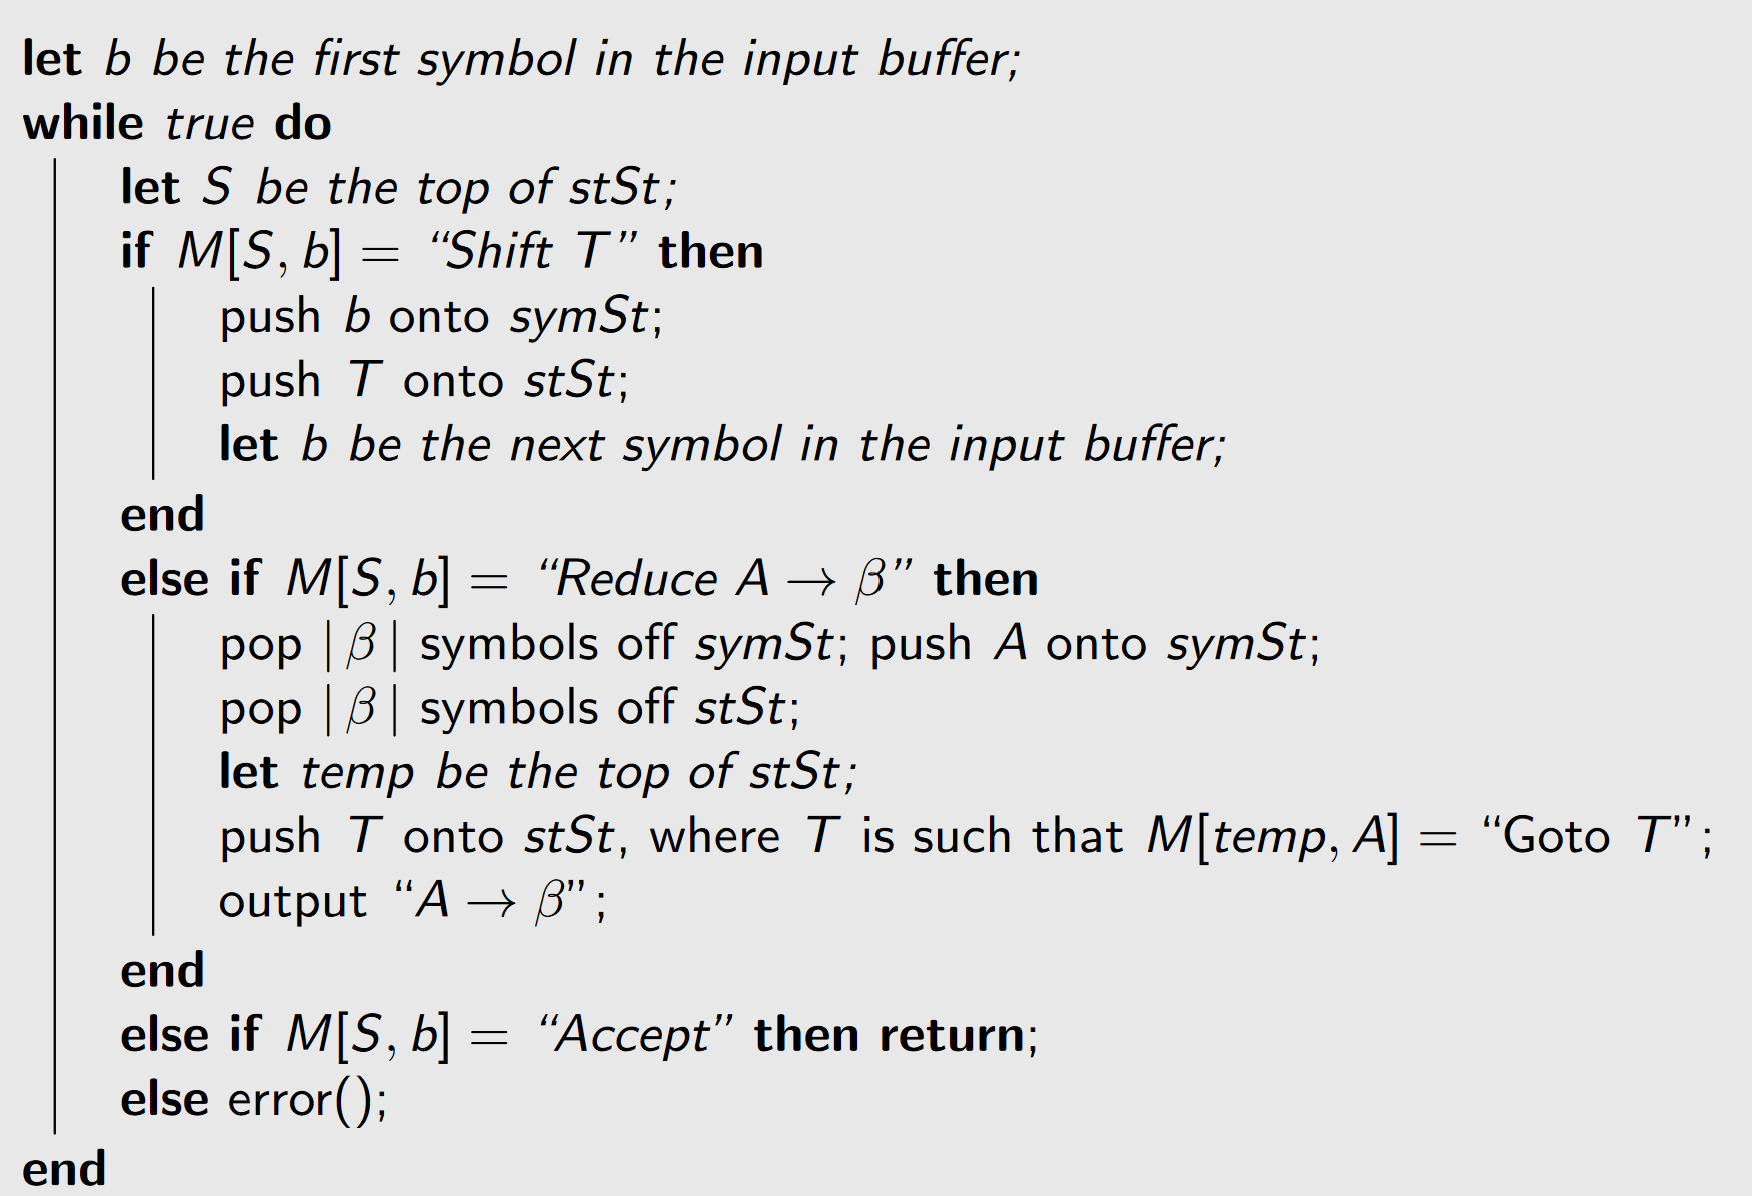
\includegraphics[width=.8\textwidth]{bottom-up-parsing-algorithm.png}
    \caption{Algoritmo di parsing Bottom-Up}
    \label{fig:bottom-up-parsing-algorithm}    
\end{figure}

Andiamo subito a mettere in pratica questo algoritmo con un esempio.

\subsubsection{Esercizio shift/reduce 1}
Consideriamo questa parola:
\begin{equation*}
    w = abbcde
\end{equation*}
Andiamo a verificare se appartiene al linguaggio generato dalla grammatica:
\begin{align}
    \label{eq:grammar-ex-sh/re-1}
    \G: S &\to aABe \\
    A &\to Abc \nonumber \\ \notag
    A &\to b \nonumber \\ \notag
    B &\to d  \nonumber \notag
\end{align}
Ne abbiamo già calcolato la tabella di parsing bottom-up in Tab.\ref{tab:parsing-table-SLR(1)parsing}.

\paragraph{Svolgimento}
La configurazione iniziale è la seguente:
\begin{align*}
    w &= abbcde\$ \\
    stSt &= 0 \\
    symSt &= 
\end{align*}
Il primo carattere che leggiamo nel buffer è \(a\), per cui cerchiamo nella tabella del parsing il contenuto della casella [0,\(a\)]; scopriamo che contiene una mossa di shift verso lo stato 2, quindi andiamo ad inserire il nuovo stato di arrivo in \(stSt\) e il carattere letto in \(symSt\):
\begin{align*}
    w &= \underline{a}bbcde\$ \\
    stSt &= 0\;2\\
    symSt &= a
\end{align*}
Ci troviamo ora nello stato 2 e leggiamo il secondo carattere della parola che è \(b\), quindi controlliamo cosa contiene la casella [2,\(b\)] della tabella di parsing. Abbiamo un'altra mossa di shift che ci fa raggiungere lo stato 4 e leggere un ennesimo carattere, e arriviamo quindi ad avere questa situazione:
\begin{align*}
    w &= \underline{ab}bcde\$ \\
    stSt &= 0\;2\;4\\
    symSt &= a\;b
\end{align*}
Ora siamo in 4 e leggiamo \(b\). La cella [4,\(b\)] ci suggerisce di compiere una mossa di reduce, nello specifico \(R: A \to b\); questo significa che compiremo due operazioni:
\begin{itemize}
    \item elimineremo tanti stati da \(stSt\) quanti gli elementi nel body della produzione;
    \item eliminiremo il body stesso da \(symSt\) e, al suo posto, inseriremo il driver della riduzione, in questo caso \(A\).
\end{itemize} 
Le nostre strutture saranno quindi valorizzate così: 
\begin{align*}
    w &= \underline{ab}bcde\$ \\
    stSt &= 0\;2\;\xout{4}\\
    symSt &= a\;A
\end{align*}
Ora però dobbiamo sostituire lo stato 4 con lo stato che è presente nella tabella in posizione [2,\(A\)], ovvero lo stato 3; la situazione si ristabilisce quindi così:
\begin{align*}
    w &= \underline{ab}bcde\$ \\
    stSt &= 0\;2\;3\\
    symSt &= a\;A
\end{align*}
Dobbiamo ancora consumare la seconda \(b\) (le mosse di reduce non consumano i caratteri), quindi ora ci troviamo nella casella [3, \(b\)],e questa ci suggerisce la mossa shift 6; vediamo cosa succede:
\begin{align*}
    w &= \underline{abb}cde\$ \\
    stSt &= 0\;2\;3\;6\\
    symSt &= a\;A\;b
\end{align*}
A questo punto la casella da guardare diventa [6,\(c\)], che ci dice shift 9, ob-la-di, ob-la-da:
\begin{align*}
    w &= \underline{abbc}de\$ \\
    stSt &= 0\;2\;3\;6\;9\\
    symSt &= a\;A\;b\;c
\end{align*}
Plot-twist! proprio mentre ci siamo abituati alla tranquillità delle mosse di shift la casella [9,\(d\)] ci lascia sbigottiti con una mossa di reduce \(R: A \to Abc\), costringendoci ad eliminare ben 3 stati da \(stSt\) e 3 caratteri da \(symSt\) e sostituendoli con una sprezzante \(A\):
\begin{align*}
    w &= \underline{abbc}de\$ \\
    stSt &= 0\;2\;\xout{3\;6\;9}\\
    symSt &= a\;\xout{A\;b\;c}A
\end{align*}
A questo punto siamo costretti a guardare in [2,\(A\)] per capire in quale stato siamo stati sballottati dal \texttt{goto}:
\begin{align*}
    w &= \underline{abbc}de\$ \\
    stSt &= 0\;2\;3\\
    symSt &= a\;A
\end{align*}
Bene, riprendiamo con la lettura: eravamo rimasti a \(d\), per cui ora controlliamo [3,\(d\)], che ci suggerisce shift 7:
\begin{align*}
    w &= \underline{abbcd}e\$ \\
    stSt &= 0\;2\;3\;7\\
    symSt &= a\;A\;d
\end{align*}
Stato 7, il prossimo carattere nel buffer è \(e\) e la casella [7,\(e\)] presenta tale riduzione \(R: B\to d\); ormai la prassi ci è nota:
\begin{align*}
    w &= \underline{abbcd}e\$ \\
    stSt &= 0\;2\;3\;\xout{7}\;5\\
    symSt &= a\;A\;\xout{d}\;B
\end{align*}
Dobbiamo ancora leggere la \(e\) e ci troviamo ora nello stato 5, e [5,\(e\)] ci dice shift 8:
\begin{align*}
    w &= \underline{abbcde}\$ \\
    stSt &= 0\;2\;3\;5\;8\\
    symSt &= a\;A\;\;B\;e
\end{align*}
Con 8 come stato e \$ come ultimo carattere ci assicuriamo una bella reduce in forma di \(R: S \to aABe\), che ci fa arrivare a questa situazione (ricordiamoci del \texttt{goto}):
\begin{align*}
    w &= \underline{abbcde}\$ \\
    stSt &= 0\;1\\
    symSt &= 
\end{align*}
Il prossimo passo è descritto dalla casella [1,\$], che ci dice Accept; questo significa che abbiamo terminato la verifica e possiamo dire, con somma pace interiore, che \(w \in \L(\G)\).

Non abbiamo solo trovato una soluzione al quesito iniziale, ma abbiamo anche ricavato i passi di derivazione che ci portano ad ottenere la parola \(w\) stessa; questi. infatti, consistono nelle riduzioni che abbiamo incontrato nel nostro cammino elencate in senso contrario:
\begin{align*}
    S &\to aABe &(aABe)\\
    B &\to d &(aAde)\\
    A &\to Abc &(aAbcde)\\
    A &\to b &(abbcde)
\end{align*}
Passiamo quindi ad un secondo esercizio, tanto più complesso quanto più completo e divertente.

\subsubsection{Esercizio shift/reduce 2}
La consegna è di costruire la parsing table SLR(1) per la seguente, ormai ben nota, grammatica:
\begin{equation}
    \label{eq:ex2-sh/re-grammar}
    E \to E+E \mid E*E \mid id
\end{equation} 
Per costruire una parsing table abbiamo prima di tutto bisogno di ricavare l'automa a stati finiti determinato da tale grammatica.
\paragraph{Ricaviamo l'automa}
\begin{enumerate}
    \item Inizializziamo lo stato 0; il suo kernel è 
    \begin{equation*}
        E' \to \cdot E
    \end{equation*}
    Di questo kernel devo calcolare la chiusura:
    \begin{align*}
        E &\to \cdot E+E \\
        E &\to \cdot E*E \\
        E &\to \cdot id
    \end{align*}
    Essendo questi gli item per lo stato 0, posso identificare due possibili transizioni (e quindi due possibili nunovi stati): \(\tau(0,E)=1 \textrm{ e } \tau(0,id)=2\).
    \item Analizziamo ora lo stato 2; il suo kernel è 
    \begin{equation*}
        E \to id.    
    \end{equation*}
    Non serve calcolare la chiusura di questo item; inoltre, tale item non comporta transizioni uscenti dallo stato 2, per cui terminiamo qui l'analisi.
    \item Passiamo al vaglio lo stato 1, il cui kernel è popolato da questi item:
    \begin{align*}
        E' &\to E.\\
        E  &\to E.+E \\
        E  &\to E.*E
    \end{align*}
    Tutti gli elementi del kernel sono già chiusi, e ci offrono queste transizioni: \(\tau(1,+)=3 \textrm{ e } \tau(1,*)=4\). Fatto ciò, abbiamo concluso l'analisi dello stato 1.
    \item Passiamo allo stato 3, il cui kernel risulta
    \begin{equation*}
        E \to E*.E
    \end{equation*}
    Tale kernel presenta però la possibilità di chiusura, per cui aggiungiamo la chiusura agli item dello stato 3, che risultano essere:
    \begin{align*}
        E &\to E*.E \\
        E &\to\ .E+E \\
        E &\to\ .E*E \\
        E &\to\ .id
    \end{align*}
    Quindi, da qui posso transizionare tramite \(E\) e tramite \(id\). La transizione per \(E\) mi porta in \(\tau(3,E)=5\), la transizione per \(id\) invece è particolare: mi porterebbe in uno stato che ha come kernel \(E \to id.\), ma quello è lo stesso kernel dello stato 2! Quindi \(\tau(3,id)=2\).
    \item Analizziamo lo stato 4, che ha per kernel
    \begin{equation*}
        E \to E*.E 
    \end{equation*}
    Si può effettuare la chiusura, quindi gli item dello stato 4 sono:
    \begin{align*}
        E &\to E*.E \\ 
        E &\to .E+E \\
        E &\to .E*E \\
        E &\to .id
    \end{align*}
    Esistono due possibili transizioni uscenti dallo stato 4: una per \(E\), che genera lo stato \(\tau(4,E)=6\), e una per \(id\), che come per il caso precedente non genera un nuovo stato ma va a finire nello stato 2.
    \item Quando analizzo lo stato 5, trovo che il kernel è
    \begin{align*}
        E &\to E+E. \\
        E &\to E.+E \\
        E &\to E.*E
    \end{align*}
    Questo non necessita di chiusura, e ci fornisce due possibili transizioni:
    \begin{itemize}
        \item quella per \(+\), che però ci porta in uno stato con kernel \({E \to E.+E}\), ovvero nello stato 3, che abbiamo già analizzato;
        \item quella per \(*\), che però ci porta in uno stato con kernel \({E \to E.*E}\), ovvero nello stato 4, che abbiamo già analizzato.
    \end{itemize}
    \item Allo stesso modo, per lo stato 6 il kernel è
    \begin{align*}
        E &\to E*E. \\
        E &\to E.+E \\
        E &\to E.*E
    \end{align*}
    e nemmeno quest necessita di chiusura, e perdipiù, attraverso le due transizioni per \(+\) e per \(*\), ci porta esattamente negli stati 3 e 4.
\end{enumerate}
Una volta terminata l'analisi degli stati e dei relativi item ci preoccupiamo di trovare quali stati contengono l'accepting item e quali stati contengono i reducing item:
\begin{itemize}
    \item l'accepting item nel metodo SLR(1) è l'item \(S' \to S.\) (ovvero \(E' \to E.\)), che nel nostro caso è contenuto nello stato 1;
    \item i reducing item sono quelli con il marker \(\cdot\) al termine di una produzione, nel nostro caso sono \(E \to id \cdot\) (stato 2), \(E \to E+E \cdot\) (stato 5) e \(E \to E*E \cdot\) (stato 6).
\end{itemize}

Per concludere la parte di costruzione dell'automa caratteristico per la nostra grammatica in Eq.\ref{eq:ex2-sh/re-grammar}, inseriamo in Fig.\ref{ex2-sh/re-automata} il disegno di tale sgorbio (scherzo, è carino, sembra un razzetto).
\begin{figure}[H]
    \center
    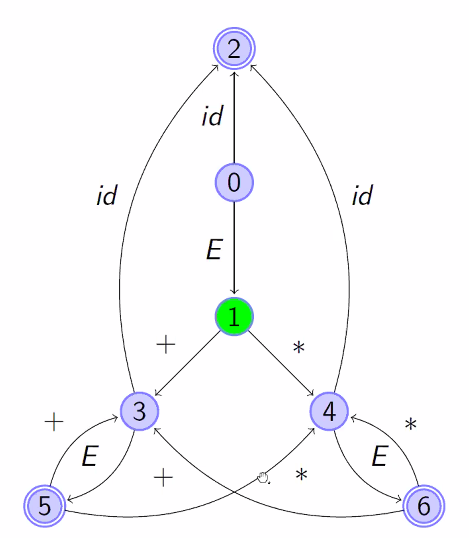
\includegraphics[width=.6\textwidth]{ex2-sh_re-automata.png}
    \caption{Automa caratteristico per la grammatica \ref{eq:ex2-sh/re-grammar}}
    \label{fig:ex2-sh/re-automata}
\end{figure}

\subsubsection{La risoluzione dei conflitti}
Quindi, partendo dalla grammatica Eq.\ref{eq:ex2-sh/re-grammar} siamo riusciti a ricavarne e l'automa caratteristico SLR(1) in Fig.\ref{fig:ex2-sh/re-automata} e i reducing items, che ricordiamo essere:
\begin{align*}
    2: E &\to id & 5: E &\to E + E \cdot & 6: E &\to E * E \cdot
\end{align*}
Tutto questo è fantastico, ma purtroppo c'è un grosso elefante nella nostra stanza. L'intrinseca ambiguità di Eq.\ref{eq:ex2-sh/re-grammar} ha un effetto collaterale piuttosto sgradevole: la sua tabella di parsing SLR(1) avrà dei conflitti, come possiamo ben vedere in Tab.\ref{tab:ex2-sh/re-table}.
\begin{figure}[H]
    \center
    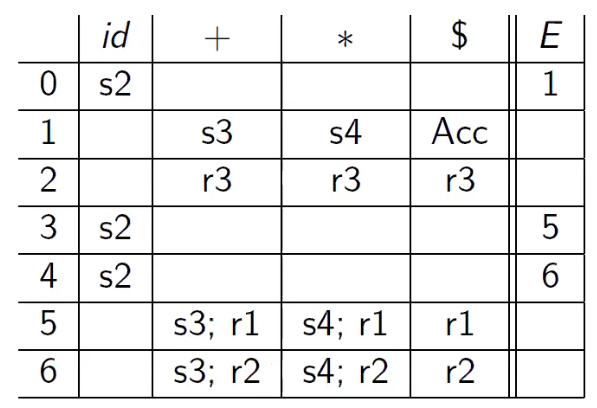
\includegraphics[width=.6\textwidth]{ex2-sh_re-table.png}
    \caption{tabella di parsing SLR(1) per la grammatica \ref{eq:ex2-sh/re-grammar}}
    \label{tab:ex2-sh/re-table}
\end{figure}
\noindent Quindi, se vogliamo perseguire la nostra ricerca di un parsing deterministico (e lo vogliamo), toccherà rimboccarsi le maniche e andare a capire come possiamo risolvere questi conflitti, non diversamente da quanto già avevamo fatto nel parsing top-down con le entries multiple defined.

I nostri conflitti sono localizzati solo in quattro situzioni, ossiamo quando ci troviamo in uno tra gli stati 5 o 6 e, contemporaneamente, troviamo in lettura un simbolo tra \(+\) o \(\ast\).
\begin{figure}[H]
    \centering
    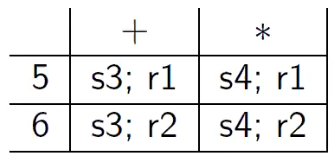
\includegraphics[width=.6\textwidth]{ex2-sh_re-table_conf.png}
    \caption{Dettaglio di Tab.\ref{tab:ex2-sh/re-grammar_conf}}
    \label{tab:ex2-sh/re-table_conf}
\end{figure}
\noindent Proviamo a capire bene qual è il punto di tutta questa situazione. Se il nostro parser si trova nello stato 5, questo vuol dire che, in testa alla nostra pila dei simboli \(symSt\), avremo necessariamente \(E + E\); possiamo vederlo facilmente, è sufficiente buttare un occhio al nostro automa caratteristico (Fig.\ref{fig:ex2-sh/re-automata}) per renderci conto che lo stato 5 è raggiungibile solo dallo stato \(3\), il quale a sua volta può essere raggiunto o dalla sequenza di stati \((0, 1)\), \((4, 6)\) o \((3, 5)\), in tutti questi casi sulla testa di \(symSt\) si troverà \(E + E\). Il discorso è del tutto analogo se passiamo allo stato 6, dove avremo la testa di \(symSt\) popolata di \(E * E\), poiché 6 è raggiungibile tramite \(\dots, 0, 1, 4, 6\), \(\dots, 4, 6, 4, 6\) oppure \(\dots, 3, 5, 4, 6\).

È chiaro che abbiamo dei conflitti quando siamo nella situazione in cui due simboli legati da un operatore sono stati già letti (\(E + E\) o \(E * E\)) e, subito dopo, leggiamo un terzo simbolo. Questo è dovuto proprio al fatto che la grammatica, nella sua ambiguità, non riesce a esprimere opportunamente né associatività, né precedenza per i due operatori.

E insomma, qual è il segreto per risolvere questi dannati conflitti? Quello che faremo (almeno in questo caso) è, per ogni cella in cui abbiamo un conflitto, scegliere manualmente quale mossa mantenere. Questa scelta pare essere in mano nostra, e nel nostro specifico esempio faremo sì che il parser finisca per conformarsi a quelle che sono le comuni regole di precedenza e associatività per \(+\) e \(*\). 

Possiamo aiutarci se pensiamo ai parse tree della nostra grammatica: gli alberi, infatti, per loro stessa costruzione, veicolano informazioni sull'annidamento dei loro elementi in maniera molto efficace, e l'annidamento può tranquillamente avere una corrispondenza diretta con la parentesizzazione. Di fatto assumendo, come facciamo noi, che i sottoalber vengano risolti prima degli alberi padri, stabiliamo delle regole di precedenza del tutto simili a quelle che si possono ottenere con una parentesizzazione.

Nello specifico, noi siamo interessati a esprimire l'associatività sinistra degli operatori \(+\) e \(*\), nonché la precedenza di \(*\) rispetto a \(+\). Diciamolo in maniera ancora più pragmatica: se guardiamo gli esempi in Fig.\ref{fig:ex2-sh_re-ptree}, vogliamo sempre avere l'albero Fig.\ref{fig:ex2-sh_re-ptree_1} al posto di Fig.\ref{fig:ex2-sh_re-ptree_2}, e vogliamo che la precedenza tra i due operatori sia tale da generare sempre parse tree come Fig.\ref{fig:ex2-sh_re-ptree_3} e Fig.\ref{fig:ex2-sh_re-ptree_4}.
\begin{figure}[H]
    \begin{minipage}[b]{.4\textwidth}
        \centering
        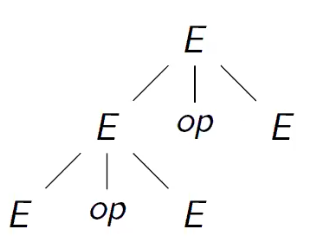
\includegraphics[width=.7\textwidth]{ex2-sh_re-ptree_1.png}
        \subcaption{Parse tree left-associativo}
        \label{fig:ex2-sh_re-ptree_1}
    \end{minipage}
    \hfill
    \begin{minipage}[b]{.4\textwidth}
        \centering
        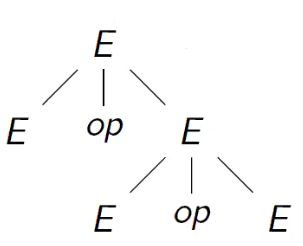
\includegraphics[width=.7\textwidth]{ex2-sh_re-ptree_2.png}
        \subcaption{Parse tree left associativo}
        \label{fig:ex2-sh_re-ptree_2}
    \end{minipage}
    
    \begin{minipage}[b]{.4\textwidth}
        \centering
        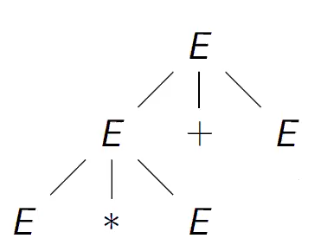
\includegraphics[width=.7\textwidth]{ex2-sh_re-ptree_3.png}
        \subcaption{Parse tree per \(E + E * E\)}
        \label{fig:ex2-sh_re-ptree_3}
    \end{minipage}
    \hfill
    \begin{minipage}[b]{.4\textwidth}
        \centering
        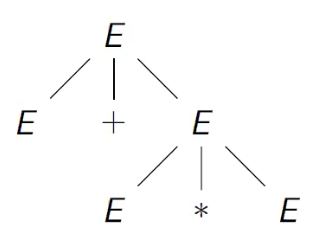
\includegraphics[width=.7\textwidth]{ex2-sh_re-ptree_4.png}
        \subcaption{Parse tree per \(E * E + E\)}
        \label{fig:ex2-sh_re-ptree_4}
    \end{minipage}
    \caption{}
    \label{fig:ex2-sh_re-ptree}
\end{figure}
In questa interpretazione possiamo vedere le mosse di reduce come una parentesizzazione, perché stiamo assegnando un padre a un determinato sottoalbero del tipo \(E + E\) o \(E * E\).

A questo punto possiamo andare ad analizzare i quattro conflitti che abbiamo trovato e, per ciascuna cella, scegliere la mossa che rende il parsing conforme alle regole che abbiamo stabilito. Tenendo a mente Tab.\ref{tab:ex2-sh/re-table_conf}, rimbocchiamoci le maniche.
\begin{itemize}
    \item \(M[5, +]\): questa è la situazione in cui la testa di \(symSt\) è popolata di \(E + E\) e in lettura troviamo un altro \(+\); gli operatori sono left-associativi, per cui vogliamo parentesizzare la testa del nostro \(symSt\) e solo dopo leggere il nuovo simbolo; ergo, la mossa che scegliamo è \(r1\).
    \item \(M[6, *]\): vediamo subito questa cella perché presenta una situazione del tutto analoga a quella appena vista;  la testa di \(symSt\) è popolata di \(E * E\) e questa volta l'operatore coinvolto è \(\ast\), che al pari di \(+\) è left-associativo, di conseguenza anche qui scegliamo la reduce \(r2\);
    \item \(M[5, *]\): torniamo adesso a parlare dello stato 5; la testa di \(symSt\) è popolata come prima, ma questa volta il lettura troviamo un simbolo \(\ast\). Questo cambia le carte in tavola, perché noi vogliamo che l'operatore \(\ast\) abbia precedenza più alta di \(+\); per ottenere questo, scegliamo la mossa di shift \(s4\), il che significa che rimandiamo la parentesizzazione della testa e proseguiamo nella lettura.
    \item \(M[6, +]\): qui abbiamo trovato \(E * E\) nella testa di \(symSt\) e ci sta arrivando un \(+\) in lettura, e ormai l'idea dovrebbe essere chiara: coerentemente con le regole di precedenza (\(\ast \prec +\)), vogliamo che la testa di \(symSt\) sia parentesizzata, per cui qui teniamo la reduce \(r2\).
\end{itemize}
\begin{figure}[H]
    \centering
    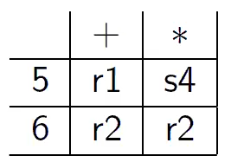
\includegraphics[width=.6\textwidth]{ex2-sh_re-table_conf_solved.png}
    \caption{Soluzione dei conflitti di Tab.\ref{tab:ex2-sh/re-grammar_conf}}
    \label{tab:ex2-sh/re-table_conf_solved}
\end{figure}
Fatto! Dopo tutto questo processo abbiamo ottenuto una tabella di parsing senza conflitti, ovvero senza entries multiple defined. Strategie di questo tipo sono abbastanza standard per le grammatiche degli operatori (non solo aritmetici, si pensi alle precedenze dell'algebra booleana); all'atto pratico, chi scrive le grammatiche (che ha studiato LFC e ha capito questi argomenti) si preoccuperà anche di predisporre delle direttive per il parser, sicché quest'ultimo abbia informazioni su quali scelte compiere in caso di conflitti.

Naturalmente, tutto questo è reso necessario dal fatto che la grammatica \(\G\) in Eq.\ref{eq:ex2-sh/re-grammar} è ambigua; se avessimo semplicemente scritto un'altra grammatica \(\G'\) non ambigua, tale che \(\L(\G) = \L(\G')\), saremmo riusciti a ottenere una tabella di parsing senza conflitti da risolvere. Dovessimo percorrere questa strada, sia chiaro che è estremamente importante che la nuova grammatica esprima correttamente le regole di precedenza e associatività che vogliamo. Guardiamo ad esempio:
\begin{align}
    \label{eq:ex2-sh/re-grammar_v2}
    \G': E &\to E + T \mid T \\
    T &\to T * id \mid id \notag
\end{align}
L'ordine con cui ho inserito le produzioni non è causale: abbiamo posizionato \(*\) in un livello di produzione inferiore a \(+\) perché, dal momento che la deriazione è rightmost e andiamo ad attraversare l'albero dal basso verso la radice (bottom-up, no?), ci assicuriamo in questo modo di parentesizzare prima tutte le occorrenze di \(\ast\); non avremmo avuto questa garanzia se avessimo inserito produzioni come, ad esempio, \(E \to T + E\). Inoltre, se ad esempio avessimo scritto \(T \to id * T\), avremmo perso la left-associatività per l'operatore \(\ast\) (ma lo stesso sarebbe successo anche per \(+\)). Il modo migliore per convincersi di queste cose (nonché il nostro suggerimento per il lettore), è quello di provare da sé a cambiare la grammatica, provare a tracciare dei parse tree e vedere cosa succede, un po'come abbiamo fatto noi qui sotto in Fig.\ref{fig:ex2-sh_re-altgrm-ptree}.
\begin{figure}[H]
    \begin{minipage}[b]{.4\textwidth}
        \centering
        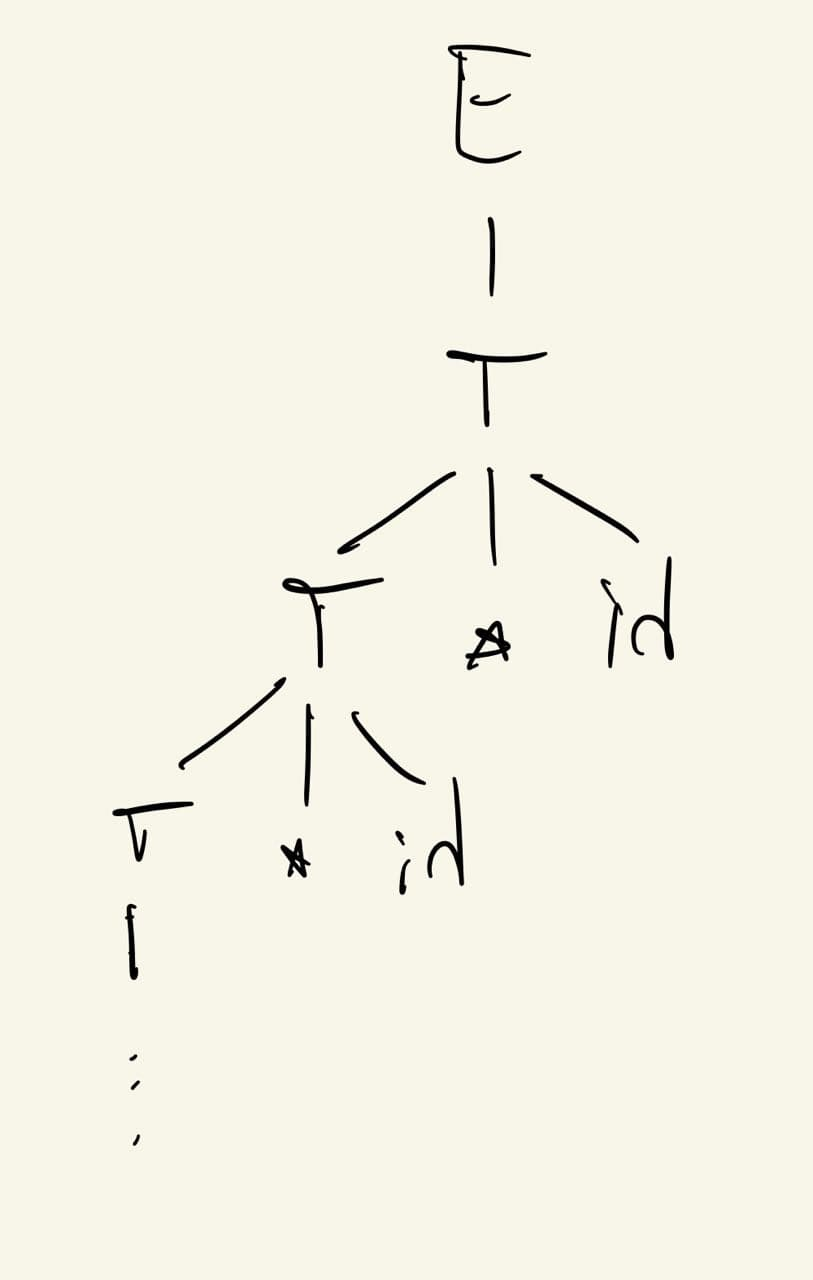
\includegraphics[width=.7\textwidth]{ex2-sh_re-altgrm-ptree_1.png}
        \subcaption{\(T \to T * id\), left-associativa (versione corretta)}
        \label{fig:ex2-sh_re-altgrm-ptree_1}
    \end{minipage}
    \hfill
    \begin{minipage}[b]{.4\textwidth}
        \centering
        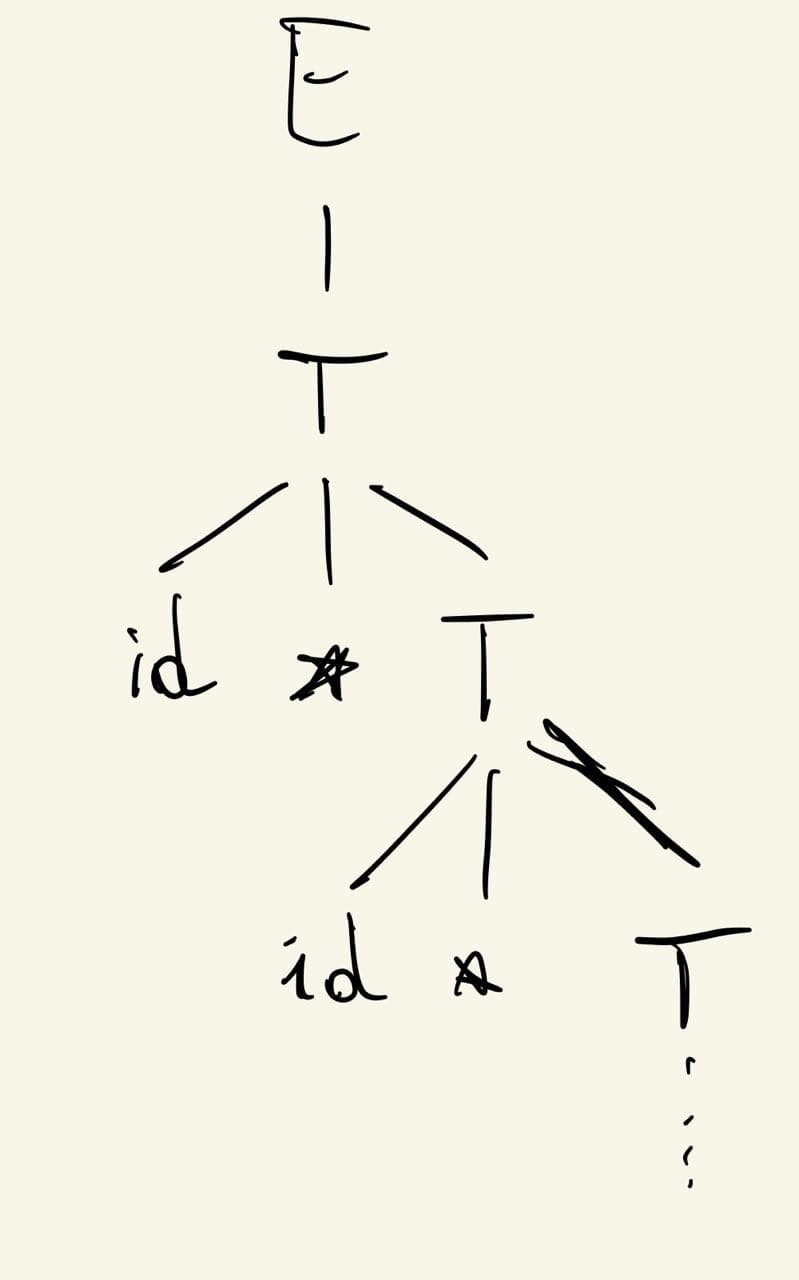
\includegraphics[width=.7\textwidth]{ex2-sh_re-altgrm-ptree_2.png}
        \subcaption{Se invece scriviamo \(T \to id * T\) perdiamo la left-associatività}
        \label{fig:ex2-sh_re-altgrm-ptree_2}
    \end{minipage}
    \caption{Esempio di come possiamo alterare Eq.\ref{eq:ex2-sh/re-grammar_v2} e vedere i cambiamenti direttamente dalla struttura dei parse trees}
    \label{fig:ex2-sh_re-altgrm-ptree}
\end{figure}

È bene far notare, inoltre, che questo procedimento ci ha portato ad aggiungere il non-terminale \(T\) alla grammatica. Certo, un non-terminale in più non ha tutto questo grande impatto sull'efficienza degli algoritmi, ma in altre situazioni la scrittura di una grammatica non ambigua che generi un linguaggio equivalente può rivelarsi davvero complicata e costosa; per questo motivo, spesso si preferisce semplicemente tenere le grammatiche ambigue e gestire i conflitti tramite direttive per il parser: il prezzo da pagare per usare una grammatica non ambigua equivalente sarebbe troppo alto.

\subsubsection{Esercizio sulla risoluzione dei conflitti}
Sia data la seguente grammatica:
\begin{align*}
    \label{eq:ex3-slr1-grammar}
    \G: S &\to aAd \mid bBd \mid aBe \mid bAe \\
    A &\to c \\
    B &\to c
\end{align*}
Il nostro obiettivo è costruire una tabella di parsing SLR(1) per la grammatica citata, e per farlo, come prima cosa, andiamo a tracciare l'automa caratteristico.
\paragraph{Ricaviamo l'automa}
\begin{enumerate}
    \item Inizializziamo lo stato 0. Il suo kernel è:
    \begin{equation*}
        S' \to \cdot S
    \end{equation*}
    Di questo kernel devo calcolare la chiusura:
    \begin{align*}
        S &\to \cdot aAd \\
    	S &\to \cdot bBd \\
    	S &\to \cdot aBe \\
    	S &\to \cdot bAe
    \end{align*}
    Essendo questi gli items per lo stato 0, posso identificare tre possibili transizioni (e quindi tre possibili nuovi stati): \(\tau(0,S)=1, \; \tau(0,a)=2 \; \textrm{e} \; \tau(0,b)=3\).
    \item Analizziamo ora lo stato 1; il suo kernel è:
    \begin{equation*}
        S' \to S \cdot    
    \end{equation*}
    Non serve calcolare la chiusura di questo item, in quanto è formata solamente da sé stesso; possiamo però evidenziare il fatto che questo è lo stato contenente l'\textbf{Accepting Item}.
    \item Analizziamo dunque lo stato 2, il cui kernel è popolato da questi item:
    \begin{align*}
        S &\to a \cdot Ad \\
        S &\to a \cdot Be
    \end{align*}
    e di cui è necessario calcolare la chiusura:
    \begin{align*}
        A &\to \cdot c \\
        B &\to \cdot c
    \end{align*}
    Anche nel caso dello stato 2 possiamo osservare la presenza di tre transizioni e quindi di tre possibili nuovi stati che sono \(\tau(2,A)=4 \textrm{, } \tau(2,B)=5 \textrm{ e } \tau(2,c)=6\).
    \item Passiamo ora allo stato 3, il cui kernel risulta:
    \begin{align*}
        S &\to b \cdot Bd \\
        S &\to b \cdot Ae
    \end{align*}
    Su questo kernel si presenta la possibilità di effettuare una chiusura, che risulta essere:
    \begin{align*}
        A &\to \cdot c \\
        B &\to \cdot c
    \end{align*}
    In questo caso è necessario prestare un po' più di attenzione, perché sebbene vi siano tre transizioni uscenti dallo stato 3, dovremo creare soltanto 2 nuovi stati: \(\tau(3,B)=7 \textrm{, } \tau(3,A)=8 \textrm{ e } \tau(3,c)=6\). Per convalidare questa affermazione è possibile osservare che il kernel dello stato 6 coinciderà esattamente con quello di questa nuova transizione.
    \item Passiamo allo stato 4, il cui kernel è:
    \begin{equation*}
        S \to aA \cdot d 
    \end{equation*}
   La chiusura di tale stato non porta nuovi elementi, tuttavia è comunque possibile definire la transizione \(\tau(4,d)\) allo stato 9.
    \item Analizzo ora lo stato 5, e il suo kernel è:
    \begin{equation*}
        S \to aB \cdot e
    \end{equation*}
    Tale stato non necessita di chiusura e ci fornisce la transizione \(\tau(5,e)\) verso lo stato 10.
    \item Procedendo come abbiamo fatto finora, il kernel per lo stato 6 è:
    \begin{align*}
        A &\to c \cdot \\
        B &\to c \cdot
    \end{align*}
    la cui chiusura non ci porta nulla di nuovo e possiamo osservare che nello stato 6 sono presenti due reducing item.
\end{enumerate}

Potremmo continuare senza fare ulteriori elucubrazioni, ma non possiamo non porre l'attenzione sullo stato appena analizzato: il fatto che vi possano essere due reducing items all'interno di un singolo stato non è necessariamente motivo di conflitti, in quanto la presenza di conflitti dipende dalla funzione di lookahead che stiamo utilizzando. Nel caso del parsing di tipo SLR(1) sappiamo che è possibile inserire un'operazione di \texttt{reduce} \(A \rightarrow \beta\) in \(M[P, Y]\) nel caso in cui \(P\) sia un stato contenente un reducing item e per tutti quei terminali \(Y \in \mathcal{LA}(P, A \rightarrow \beta) = follow(A)\): in questo caso \(follow(A) = follow(B) = \{d, e\}\), il che significa che avremo almeno due celle dove sono presenti dei conflitti nella nostra parsing table finale.

Tuttavia, in questo caso la colpa non è della grammatica, ma va ricercata piuttosto nel tipo di parsing adoperato, fin troppo grosolano: invece di accorpare tutto all'interno di un singolo stato (riguardiamo lo stato 6), non sarebbe meglio avere due stati differenti? 

Ovviamente stato 2 e lo stato 3 "ricordano" delle informazioni differenti e per poter risolvere questa indecisione è necessario considerare in quale modo si è arrivati all'item di riduzione. Ad esempio, nel caso in cui avessimo letto fino ad ora la parola \(ac\) e ci trovassimo quindi in dubbio su che tipo di operazione di reduce effettuare, basterebbe semplicemente poter osservare quale fosse il prossimo simbolo: 
\begin{itemize}
    \item effettuiamo \texttt{reduce} \(A \to c\) nel caso in cui il prossimo simbolo sia \(d\) in quanto è possibile derivare da \(S\) solamente una parola del tipo \(aAd\);
    \item effettuiamo \texttt{reduce} \(B \to c\) nel caso in cui il prossimo simbolo sia \(e\) in quanto è possibile derivare da \(S\) solamente una parola del tipo \(aBe\).
\end{itemize}

\subsection{LR(1)-items}
Per poter ottenere quanto detto andremo a utilizzare gli LR(1)-items, che hanno questa forma:
\begin{equation}
    \label{lr0}
    [A \to \alpha \cdot \beta, \Delta]
\end{equation}
Dove \(\Delta\) è detto \textbf{lookahead-set}.

Quando applicata a \([A \to \alpha \cdot B \beta, \Delta]\), la \(closure_1(\_)\) rifinisce la \(closure_0(\_)\) propagando i simboli che seguono \(B\) nella produzione \(A \to \alpha \cdot B \beta\) agli items che vengono aggiunti per fare l'operazione di chiusura rispetto a \(B\).

\subsection{Chiusure di insiemi di LR(1)-item}
Come facciamo a calcolare la chiusura degli insiemi di LR(1)-items? Iniziamo dunque fornendo la definizione per la computazione a punto fisso:
\begin{definition}
    \label{def:lr1-closure}
    Sia \(P\) un insieme di item LR(1)-item, la \(closure_1(P)\) identifica il più piccolo insieme di item, con il più piccolo lookahead-set, che soddisfa la seguente equazione:
    \begin{equation*}
        closure_1(P) = P \cup \{[B \rightarrow \cdot \gamma, \Gamma] : [A \rightarrow \alpha \cdot B \beta, \Delta] \in closure_1(P) \textrm{ and } B \rightarrow \gamma \in \P' \textrm{ and } first(\beta \Delta) \subseteq \Gamma\}
    \end{equation*}  
    dove \(first(\beta \Delta) = \cup_{d \in \Delta} first(\beta d)\).
\end{definition}

\subsubsection{Esesercizio 1: computazione \(closure_1(P)\)}
Facendo riferimento alla grammatica dell'esercizio precedente (Eq.\ref{eq:ex3-slr1-grammar}), calcolare la chiusura \(closure_1(\{[S' \to \cdot S, \{\$\}]\})\): questa inizializzazione sottolinea il fatto che, che una volta che avremo raggiunto il particolare stato in cui avremo l'accepting item \(S' \to \cdot S\), vorremo vedere il \$ che viene utilizzato come terminatore per definire una parola appartenente al linguaggio. Quindi, che si fa ora?

Secondo la Def.\ref{def:lr1-closure}, l'unico item che appartiene alla chiusura è \([S' \to \cdot S, \{\$\}] = [A \rightarrow \alpha \cdot B \beta, \Delta]\),e dovremo aggiungere a questa chiusura degli item nella forma \([B \rightarrow \cdot \gamma, \Gamma]\), per cui:
\begin{itemize}
    \item la prima componente di questa coppia corrisponde a tutte quelle produzioni nella grammatica che hanno forma \(B \rightarrow \gamma\);
    \item  la seconda componente invece (\(\Gamma\)) sarà un insieme contenente tanti elementi quanti sono i \(first(\beta \Delta)\), dove \(\Delta\) fa riferimento al lookahead-set dell'item che stiamo considerando, mentre \(\beta\) è tutto ciò che segue il non-terminale B.
\end{itemize} 
Nel caso dell'item \([S' \to \cdot S, \{\$\}]\), dunque, possiamo affermare che \(\Delta = \{\$\} \textrm{ e } \beta = \varepsilon\) e, di conseguenza, \(first(\varepsilon \$) = first(\$) = \{\$\} \subseteq \Gamma\). Gli item che otterremo da \(closure_1(\{[S' \to \cdot S, \{\$\}]\})\) saranno dunque:
\begin{align*}
    [S' &\to \cdot S, \{\$\}] \\
    [S &\to \cdot aAd, \{\$\}] \\
	[S &\to \cdot bBd, \{\$\}] \\
	[S &\to \cdot aBe, \{\$\}] \\
	[S &\to \cdot bAe, \{\$\}]
\end{align*}
Quanto abbiamo appena ottenuto è la chiusura dell'insieme che costituisce lo stato 0 del nostro automa caratteristico di tipo LR(1).

Notare che la componente del lookahead-set è utile per le riduzioni, mentre nel caso delle transizioni non fornirà alcuna informazione aggiuntiva, per cui il procedimento rimarrà sotto quel punto di vista inalterato. Di conseguenza, possiamo affermare la presenza, come nel caso iniziale, di tre transizioni che portano a tre stati differenti: \(\tau(0,S)=1 \textrm{, } \tau(0,a)=2 \textrm{ e } \tau(0,b)=3\). A questo punto è possibile procedere come abbiamo sempre fatto prestando attenzione alla computazione delle \(closure_1(S)\):
\begin{enumerate}
    \item Proseguiamo osservando lo stato 1. Il suo kernel è:
    \begin{equation*}
        [S' \to S \cdot, \{\$\}]
    \end{equation*}
    dobbiamo dunque calcolare \(closure_1(\{[S' \to S \cdot, \{\$\}]\})\), per cui sappiamo che \(B = \varepsilon\) e dunque non possiamo fare altro se non appuntarci che lo stato 1 contiene l'Accepting Item.
    \item Analizziamo dunque lo stato 2, il cui kernel è popolato da questi item:
    \begin{align*}
        [S &\to a \cdot Ad, \{\$\}] \\
        [S &\to a \cdot Be, \{\$\}]
    \end{align*}
    per cui sappiamo che, nel caso in cui esista una produzione con A come driver, si ha che \(B = A, \beta = d, \Delta = \{\$\}\) (e quindi \(\Gamma_A = first(\beta \Delta) = first(d\$)\)), mentre, nel caso in cui esista una produzione con B come driver, si ha che \(B = B, \beta = e, \Delta = \{\$\}\) (e quindi \(\Gamma_B = first(\beta \Delta) = first(e\$)\)) . Calcoliamo dunque la chiusura:
    \begin{align*}
        [A &\to \cdot c, \{d\}] \\
        [B &\to \cdot c, \{e\}]
    \end{align*}
    Come succedeva nell'esempio con il parsing LR(0), nello stato 2 possiamo osservare la presenza di tre transizioni e quindi di tre possibili nuovi stati che sono \(\tau(2,A)=4 \textrm{, } \tau(2,B)=5 \textrm{ e } \tau(2,c)=6\).
    \item[...]
    \item[6.] Ovviamente la parte interessante dell'esercizio è verificare se siamo riusciti a risolvere il conflitto che occorreva nel parsing SLR(1). In modo pressoché analogo a quanto accadeva abbiamo che il kernel per lo stato 6 è :
    \begin{align*}
        [A &\to c \cdot, \{d\}] \\
        [B &\to c \cdot, \{e\}]
    \end{align*}
    Anche questa volta lo stato è caratterizzato dalla presenza di due reducing item, ma in questo caso questi non portano a dei conflitti,perché sappiamo che dovremo applicare un'operazione di \texttt{reduce} \(A \to c\) solamente nel caso in cui il prossimo elemento in input sia \(d\), mentre un'operazione di \texttt{reduce} \(A \to c\) nel caso in cui sia invece \(e\).
\end{enumerate}

\subsubsection{Esesrcizio 2: computazione \(closure_1(P)\)}
Sia data la seguente grammatica:
\begin{align}
    \label{}
    \G: S &\to L=R \mid R \\
    L &\to *R \mid id \\ \notag
    R &\to L \notag
\end{align}
Inizializziamo lo stato 0 ponendo come suo kernel:
\begin{equation}
    [S' \to \cdot S, \{\$\}]
\end{equation}
Calcoliamo \(closure_1(0)\) (ci fermiamo dopo la prima iterazione):
\begin{align*}
    [S &\to \cdot L = R, \{\$\}] \\
    [S &\to \cdot R, \{\$\}]
\end{align*}
Un risultato di questo tipo è ancora una volta osservabile dal fatto che l'unico elemento presente all'interno della chiusura è \([S' \to \cdot S, \{\$\}]\), dunque \(B = S \texttt{, } \beta = \varepsilon \texttt{, } \Delta = \{\$\}\) (e quindi \(\Gamma = first(\beta \Delta) = first(\varepsilon \$) = \{\$\}\)).

A questo punto la chiusura non è completa in quando abbiamo aggiunto due elementi che possono essere presi in considerazione nella definizione ricorsiva della chiusura: selezioniamo dunque \([S \to \cdot L = R, \{\$\}]\) e proseguiamo nella procedura considerando \(B = L \texttt{, } \beta = \{=\} \texttt{, } \Delta = \{\$\}\) (e quindi \(\Gamma = first(\beta \Delta) = first(\{=\} \$) = \{=\}\)), ottenendo:
\begin{align*}
    [L &\to \cdot *R, \{=\}] \\
    [L &\to \cdot id, \{=\}]
\end{align*}
Allo stesso modo è possibile continuare con \([S \to \cdot R, \{\$\}]\) ponendo \(B = R \texttt{, } \beta = \{\varepsilon\} \texttt{, } \Delta = \{\$\}\) (e quindi \(\Gamma = first(\beta \Delta) = first(\varepsilon \$) = \{\$\}\)), ottenendo:
\begin{align*}
    [R &\to \cdot L, \{\$\}]
\end{align*}
Nonostante la produzione con driver \(L\) sia già stata analizzata, è necessario eseguire nuovamente la sua chiusura in quanto ha un lookahed-set differente, il che ci porta ad inserire:
\begin{align*}
    [L &\to \cdot *R, \{\$\}] \\
    [L &\to \cdot id, \{\$\}]
\end{align*}
Visto che però avevamo già inserito due LR(1)-item con lo stesso LR(0)-item possiamo semplicemente accrescere i lookahead-set corrispondenti. Il risultato finale per lo stato iniziale può essere dunque riscritto nel seguente modo:
\begin{align*}
    [S' &\to \cdot S, \{\$\}] \\
    [S &\to \cdot L = R, \{\$\}] \\
    [S &\to \cdot R, \{\$\}] \\
    [L &\to \cdot *R, \{\$, =\}] \\
    [L &\to \cdot id, \{\$, =\}] \\
    [R &\to \cdot L, \{\$\}]
\end{align*}

\end{document}